\documentclass{article}
\setlength{\emergencystretch}{3em}
\usepackage[utf8]{inputenc}
\usepackage{amsmath}
\usepackage{amssymb}
\usepackage{geometry}
\usepackage{graphicx}
\usepackage{float}
\usepackage{tikz}
\usepackage{subcaption}
\usepackage{tabularx}
\usepackage{booktabs}
\usepackage[round]{natbib}
\usepackage{enumitem}
\usepackage{tcolorbox}
\tcbuselibrary{breakable}
\tcbset{
  boxstyle/.style={
    colback=gray!4,
    colframe=black!35,
    fonttitle=\bfseries,
    coltitle=white,
    colbacktitle=black!55,
    breakable,
    before skip=1.4em,
    after skip=1.4em,
    left=6pt, right=6pt, top=6pt, bottom=6pt
  }
}

\usetikzlibrary{shapes.geometric, arrows, positioning, calc, patterns, decorations.pathreplacing}

\geometry{a4paper, margin=1in}
\setlength{\parindent}{0pt}
\setlength{\parskip}{0.8em}

% Supplement-specific numbering
\renewcommand{\thefigure}{S\arabic{figure}}
\renewcommand{\thetable}{S\arabic{table}}
\renewcommand{\theequation}{S\arabic{equation}}

\title{Supplementary Material for:\\[0.5em]
Flooding the filter: a game-theoretic model of AI, submission pressure, and quality collapse}
\author{Yuhui Fang}
\date{\today}

\begin{document}

\maketitle

\begin{figure}[H]
\centering
\resizebox{\textwidth}{!}{%
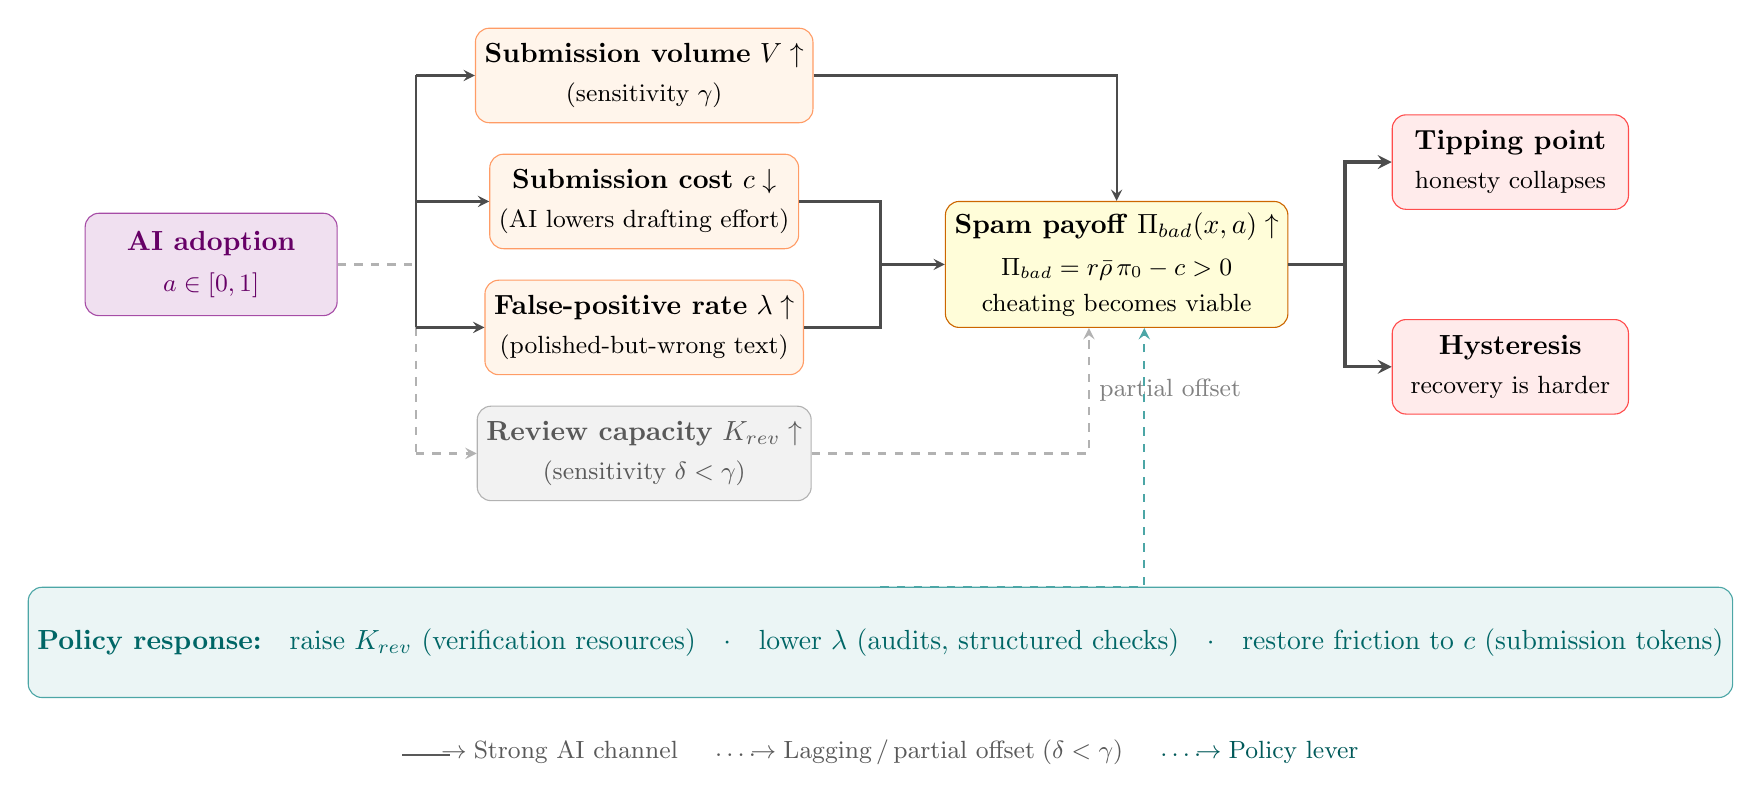
\begin{tikzpicture}[
    >=stealth,
    font=\normalsize,
    ai/.style={
        rectangle, rounded corners=5pt,
        draw=violet!70, fill=violet!12,
        minimum width=3.2cm, minimum height=1.3cm,
        align=center, text=violet!80!black
    },
    channel/.style={
        rectangle, rounded corners=5pt,
        draw=orange!70!red!60, fill=orange!8,
        minimum width=3.8cm, minimum height=1.2cm,
        align=center
    },
    lag/.style={
        rectangle, rounded corners=5pt,
        draw=gray!60, fill=gray!10,
        minimum width=3.8cm, minimum height=1.2cm,
        align=center, text=gray!70!black
    },
    pibad/.style={
        rectangle, rounded corners=5pt,
        draw=orange!80!black, fill=yellow!15,
        minimum width=4.0cm, minimum height=1.6cm,
        align=center
    },
    outcome/.style={
        rectangle, rounded corners=5pt,
        draw=red!70, fill=red!8,
        minimum width=3.0cm, minimum height=1.2cm,
        align=center
    },
    policy/.style={
        rectangle, rounded corners=5pt,
        draw=teal!70, fill=teal!8,
        minimum width=12.0cm, minimum height=1.4cm,
        align=center, text=teal!80!black
    },
    strong/.style={thick, ->, black!70},
    weak/.style={thick, ->, dashed, gray!60},
    plcy/.style={thick, ->, dashed, teal!70}
]

\node (ai) [ai] at (0,0)
    {\textbf{AI adoption}\\[3pt]{\small $a \in [0,1]$}};

\node (vup)   [channel] at (5.5, 2.4)
    {\textbf{Submission volume} $V \uparrow$\\[2pt]{\small (sensitivity $\gamma$)}};
\node (cdown) [channel] at (5.5, 0.8)
    {\textbf{Submission cost} $c \downarrow$\\[2pt]{\small (AI lowers drafting effort)}};
\node (lup)   [channel] at (5.5,-0.8)
    {\textbf{False-positive rate} $\lambda \uparrow$\\[2pt]{\small (polished-but-wrong text)}};
\node (krev)  [lag]     at (5.5,-2.4)
    {\textbf{Review capacity} $K_{rev} \uparrow$\\[2pt]{\small (sensitivity $\delta < \gamma$)}};

\node (pibad) [pibad] at (11.5, 0)
    {\textbf{Spam payoff} $\Pi_{bad}(x,a) \uparrow$\\[3pt]
     {\small $\Pi_{bad} = r\bar{\rho}\,\pi_0 - c > 0$}\\[1pt]
     {\small cheating becomes viable}};

\node (tip)  [outcome] at (16.5, 1.3)
    {\textbf{Tipping point}\\[2pt]{\small honesty collapses}};
\node (hyst) [outcome] at (16.5,-1.3)
    {\textbf{Hysteresis}\\[2pt]{\small recovery is harder}};

\node (policy) [policy] at (8.5,-4.8)
    {\textbf{Policy response:}\quad
     raise $K_{rev}$ (verification resources)\quad$\cdot$\quad
     lower $\lambda$ (audits, structured checks)\quad$\cdot$\quad
     restore friction to $c$ (submission tokens)};

\def\busA{2.6}
\def\busB{8.5}
\def\busC{14.4}

\draw[weak, -] (ai.east) -- (\busA, 0);
\draw[strong, -] (\busA, 2.4) -- (\busA, -0.8);
\draw[weak, -]   (\busA, -0.8) -- (\busA, -2.4);
\draw[strong] (\busA, 2.4) -- (vup.west);
\draw[strong] (\busA, 0.8) -- (cdown.west);
\draw[strong] (\busA, -0.8) -- (lup.west);
\draw[weak]   (\busA, -2.4) -- (krev.west);

\draw[strong] (vup.east) -| (pibad.north);
\draw[weak]   (krev.east) -| node[pos=0.75, right, font=\small, text=gray] {partial offset} ([xshift=-10pt]pibad.south);
\draw[strong, -] (cdown.east) -| (\busB, 0);
\draw[strong, -] (lup.east)   -| (\busB, 0);
\draw[strong] (\busB, 0) -- (pibad.west);

\draw[strong, line width=1.2pt, -] (pibad.east) -- (\busC, 0);
\draw[strong, line width=1.2pt] (\busC, 0) |- (tip.west);
\draw[strong, line width=1.2pt] (\busC, 0) |- (hyst.west);

\draw[plcy] (policy.north) -| ([xshift=10pt]pibad.south);

\node (legend) [font=\small, text=black!65] at (8.5, -6.2)
    {\raisebox{1pt}{\rule{0.6cm}{0.8pt}}$\!\!\rightarrow$\;Strong AI channel
     \quad
     \raisebox{1pt}{\makebox[0.6cm]{\dotfill}}$\!\!\rightarrow$\;Lagging\,/\,partial offset\;($\delta<\gamma$)
     \quad
     \textcolor{teal!70!black}{\raisebox{1pt}{\makebox[0.6cm]{\dotfill}}$\!\!\rightarrow$}\;\textcolor{teal!70!black}{Policy lever}};

\end{tikzpicture}%
}
\caption{\textbf{Mechanism diagram: AI as an asymmetric shock to the publication system.}
AI adoption ($a$) raises submission volume ($V$, sensitivity $\gamma$) and lowers
drafting cost ($c$), while polished AI text increases the false-positive rate ($\lambda$).
Review capacity ($K_{rev}$) rises more slowly (sensitivity $\delta < \gamma$), so the
partial offset from AI-assisted reviewing is insufficient to prevent congestion.
Together, these shifts raise the profitability of submitting low-quality work
($\Pi_{bad} = r\bar{\rho}\,\pi_0 - c$), pushing the system towards a tipping point
and widening the gap between the collapse and recovery thresholds (hysteresis).
Effective policy must raise $K_{rev}$, reduce $\lambda$, and restore friction to $c$
(dashed teal arrow).}
\label{fig:mechanism}
\end{figure}

\begin{figure}[H]
    \centering
    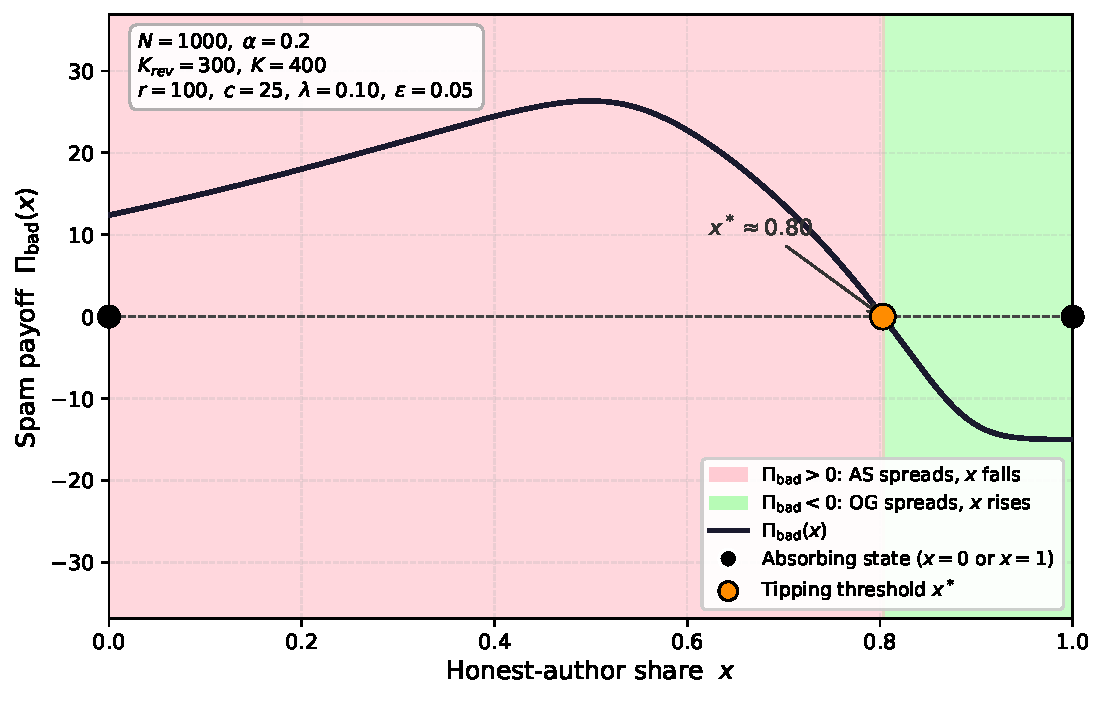
\includegraphics[width=0.9\textwidth]{polynomial_graph_1.pdf}
    \caption{\textbf{Phase portrait under pre-AI parameters ($a = 0$, bistability).}
    The curve plots $\Pi_{bad}(x, 0)$, the net payoff from submitting a weak paper, against the honest-author share $x$.
    Parameters: $N=1000$, $K_{rev}=300$, $K=400$, $r=100$, $c=25$, $\lambda=0.1$, $a=0$.
    Red shading: $\Pi_{bad}>0$, so AS spreads and $x$ falls.
    Blue shading: $\Pi_{bad}<0$, so OG spreads and $x$ rises.
    Two long-run outcomes coexist---full honesty ($x=1$) and full corruption ($x=0$)---separated by an unstable tipping threshold at $x^*\approx 0.80$ (orange marker).
    Setting $a > 0$ shifts the curve upward, narrowing the basin of attraction around honesty.}
    \label{fig:replicator_dynamics}
\end{figure}

\appendix

\section{Proofs of Propositions~1--4}
\label{app:proofs}

The four propositions in the main text characterise how the spam payoff $\Pi_{\mathit{bad}}(x,a)$ responds to the AI adoption parameter~$a$ and to the four institutional levers $\lambda$, $K_{\mathit{rev}}$, $c$, and $K$.
This appendix provides complete formal derivations.
We first collect notation and establish three lemmas that are used repeatedly across the proofs.

\paragraph{Notation.}

Throughout, $x \in [0,1]$ is the share of selective (OG) authors and $a \in [0,1]$ is the AI adoption intensity.
Define:
\begin{align*}
  V_0(x)              &\;\equiv\; N\bigl[1-(1-\alpha)x\bigr]
    && \text{baseline submission volume (at $a=0$),}\\
  V(x,a)              &\;=\; V_0(x)(1+\gamma a)
    && \text{total submission volume,}\\
  K_{\mathit{rev}}(a) &\;=\; K_{\mathit{rev}}(0)(1+\delta a)
    && \text{review capacity,}\\
  \eta(x,a)           &\;=\; \min\!\Bigl(1,\;\tfrac{K_{\mathit{rev}}(a)}{V(x,a)}\Bigr)
    && \text{screening intensity,}\\
  \pi_0(x,a)          &\;=\; 1 - \eta(x,a)\bigl(1-\lambda(a)\bigr)
    && \text{bad-paper pass rate,}\\
  \pi_1(x,a)          &\;=\; 1 - \eta(x,a)\,\varepsilon
    && \text{good-paper pass rate,}\\
  M(x,a)              &\;=\; (1+\gamma a)\bigl[N\alpha\,\pi_1(x,a) + N(1-\alpha)(1-x)\,\pi_0(x,a)\bigr]
    && \text{peer-accepted pool,}\\
  \bar\rho(x,a)       &\;=\; \min\!\Bigl(1,\;\tfrac{K}{M(x,a)}\Bigr)
    && \text{rationing probability,}\\
  \Pi_{\mathit{bad}}(x,a) &\;=\; r\,\bar\rho(x,a)\,\pi_0(x,a) - c(a)
    && \text{spam payoff.}
\end{align*}

We work throughout under the \textbf{AI asymmetry assumption} $\gamma > \delta \geq 0$ and the parametric assumptions $\mu \geq 0$, $\phi \in (0,1)$, $r, c_0 > 0$.
We also impose the \textbf{discriminatory filter condition}:
\begin{equation}
  \label{eq:app_filter}
  \lambda(a) + \varepsilon < 1 \qquad \text{for all } a \in [0,1].
\end{equation}
This states that peer review rejects bad papers at a strictly higher rate than it falsely rejects good ones, i.e.\ the filter is better than random.
The proofs split into three cases based on which capacity constraints are binding:
\begin{itemize}
  \item \textbf{Case~I} (uncongested): $V(x,a) \leq K_{\mathit{rev}}(a)$, so $\eta = 1$.
  \item \textbf{Case~II} (congested, unrationed): $V > K_{\mathit{rev}}$ and $M \leq K$, so $\eta < 1$ and $\bar\rho = 1$.
  \item \textbf{Case~III} (congested and rationed): $V > K_{\mathit{rev}}$ and $M > K$, so $\eta < 1$ and $\bar\rho = K/M < 1$.
\end{itemize}

\paragraph{Lemma A.1 (Screening intensity falls with $a$).}

\textit{In Cases~II and~III:}
\begin{equation}
  \label{eq:app_deta}
  \frac{\partial\eta}{\partial a}
  = \frac{K_{\mathit{rev}}(0)\,(\delta-\gamma)}{V_0(x)\,(1+\gamma a)^2} < 0.
\end{equation}

\noindent\textit{Proof.}
Substitute $K_{\mathit{rev}}(a) = K_{\mathit{rev}}(0)(1+\delta a)$ and $V(x,a) = V_0(x)(1+\gamma a)$ into $\eta = K_{\mathit{rev}}(a)/V(x,a)$ and differentiate with respect to $a$ using the quotient rule.
The numerator of the result is $K_{\mathit{rev}}(0)[\delta(1+\gamma a) - \gamma(1+\delta a)] = K_{\mathit{rev}}(0)(\delta - \gamma) < 0$ since $\gamma > \delta$.
\hfill$\square$

\paragraph{Lemma A.2 (Both pass rates rise with $a$).}

\textit{In Cases~II and~III, writing $\dot\eta \equiv \partial\eta/\partial a < 0$:}
\begin{align}
  \frac{\partial\pi_0}{\partial a} &= -\dot\eta\,(1-\lambda) + \eta\,\mu > 0,
    \label{eq:app_dpi0} \\
  \frac{\partial\pi_1}{\partial a} &= -\dot\eta\,\varepsilon > 0.
    \label{eq:app_dpi1}
\end{align}

\noindent\textit{Proof.}
Differentiate $\pi_0 = 1 - \eta(1-\lambda(a))$ with respect to $a$.
The product rule gives $-\dot\eta(1-\lambda) + \eta\,d\lambda/da = -\dot\eta(1-\lambda) + \eta\mu$.
Both terms are non-negative because $\dot\eta < 0$, $1-\lambda > 0$, $\eta > 0$, and $\mu \geq 0$; the first term is strictly positive.
Differentiate $\pi_1 = 1 - \eta\varepsilon$ with respect to $a$; since $\varepsilon$ is a fixed parameter, $\partial\pi_1/\partial a = -\dot\eta\varepsilon > 0$.
\hfill$\square$

\paragraph{Lemma A.3 (Bad-paper advantage grows with $a$).}

\textit{In Cases~II and~III, (i) the ratio $\pi_0/\pi_1$ is strictly increasing in $a$:}
\begin{equation}
  \frac{d}{da}\!\left(\frac{\pi_0}{\pi_1}\right) > 0;
  \label{eq:app_ratio}
\end{equation}
\textit{and (ii) defining the base pool $M_0 \equiv N\alpha\pi_1 + N(1-\alpha)(1-x)\pi_0$, the following key inequality holds:}
\begin{equation}
  M_0\,\frac{\partial\pi_0}{\partial a} - \pi_0\,\frac{\partial M_0}{\partial a}
  = N\alpha\!\left(\pi_1\,\frac{\partial\pi_0}{\partial a}
     - \pi_0\,\frac{\partial\pi_1}{\partial a}\right) > 0.
  \label{eq:app_key}
\end{equation}

\noindent\textit{Proof of part (i).}
By the quotient rule, the sign of $d(\pi_0/\pi_1)/da$ equals the sign of $\pi_1\,\partial\pi_0/\partial a - \pi_0\,\partial\pi_1/\partial a$.
Substituting \eqref{eq:app_dpi0}--\eqref{eq:app_dpi1}:
\begin{align*}
  &\pi_1\,\frac{\partial\pi_0}{\partial a} - \pi_0\,\frac{\partial\pi_1}{\partial a} \\
  &\quad= (1-\eta\varepsilon)\bigl[-\dot\eta(1-\lambda)+\eta\mu\bigr]
    - (1-\eta(1-\lambda))\bigl[-\dot\eta\varepsilon\bigr] \\
  &\quad= \dot\eta\Bigl[\varepsilon\bigl(1-\eta(1-\lambda)\bigr)
          - (1-\lambda)\bigl(1-\eta\varepsilon\bigr)\Bigr]
       + \eta\mu(1-\eta\varepsilon).
\end{align*}
Expand the bracket in the first term:
\[
  \varepsilon\bigl(1-\eta(1-\lambda)\bigr) - (1-\lambda)\bigl(1-\eta\varepsilon\bigr)
  = \varepsilon - (1-\lambda)
  = \varepsilon + \lambda - 1 < 0,
\]
where the last inequality uses condition~\eqref{eq:app_filter}.
Since $\dot\eta < 0$ and $(\varepsilon+\lambda-1) < 0$, the first term $\dot\eta(\varepsilon+\lambda-1) > 0$.
The second term $\eta\mu(1-\eta\varepsilon) \geq 0$.
Therefore $\pi_1\,\partial\pi_0/\partial a - \pi_0\,\partial\pi_1/\partial a > 0$ and $d(\pi_0/\pi_1)/da > 0$.

\medskip\noindent\textit{Proof of part (ii).}
Expand $M_0\,\partial\pi_0/\partial a - \pi_0\,\partial M_0/\partial a$ using $M_0 = N\alpha\pi_1 + N(1-\alpha)(1-x)\pi_0$ and $\partial M_0/\partial a = N\alpha\,\partial\pi_1/\partial a + N(1-\alpha)(1-x)\,\partial\pi_0/\partial a$:
\begin{align*}
  &M_0\,\frac{\partial\pi_0}{\partial a} - \pi_0\,\frac{\partial M_0}{\partial a} \\
  &= \bigl[N\alpha\pi_1 + N(1-\alpha)(1-x)\pi_0\bigr]\frac{\partial\pi_0}{\partial a}
     - \pi_0\Bigl[N\alpha\frac{\partial\pi_1}{\partial a}
       + N(1-\alpha)(1-x)\frac{\partial\pi_0}{\partial a}\Bigr] \\
  &= N\alpha\!\left(\pi_1\,\frac{\partial\pi_0}{\partial a}
     - \pi_0\,\frac{\partial\pi_1}{\partial a}\right).
\end{align*}
The $N(1-\alpha)(1-x)\pi_0\,\partial\pi_0/\partial a$ terms cancel exactly, leaving $N\alpha(\pi_1\,\partial\pi_0/\partial a - \pi_0\,\partial\pi_1/\partial a) = N\alpha\pi_1^2\,(d/da)(\pi_0/\pi_1) > 0$ by part (i).
\hfill$\square$

\bigskip

\paragraph{Proof of Proposition~1 (Monotone Destabilisation).}

\noindent\textit{Claim: Under $\gamma > \delta \geq 0$, $\mu \geq 0$, $\phi > 0$, $\Pi_{\mathit{bad}}(x,a)$ is strictly increasing in $a$ for every $x \in (0,1)$.
Consequently, the GH region in $(K_{\mathit{rev}},K)$ space shrinks weakly as $a$ rises, and there exists a finite threshold $a^* \in (0,1]$ above which no $(K_{\mathit{rev}},K)$ pair sustains GH without additional institutional intervention.}

\medskip\noindent\textbf{Step 1: Show $\partial\Pi_{\mathit{bad}}/\partial a > 0$ in each case.}

\noindent\textbf{Case~I} ($\eta=1$, $\bar\rho=1$):
In the uncongested, unrationed region $\Pi_{\mathit{bad}} = r\lambda(a) - c(a)$, so $\partial\Pi_{\mathit{bad}}/\partial a = r\mu + c_0\phi > 0$.

\noindent\textbf{Case~II} ($\eta<1$, $\bar\rho=1$):
$\Pi_{\mathit{bad}} = r\pi_0(x,a) - c(a)$, so $\partial\Pi_{\mathit{bad}}/\partial a = r\,\partial\pi_0/\partial a + c_0\phi > 0$ by Lemma~A.2 and $\phi > 0$.

\noindent\textbf{Case~III} ($\eta<1$, $\bar\rho<1$):
Writing $M_0 \equiv N\alpha\pi_1 + N(1-\alpha)(1-x)\pi_0$ and $M = (1+\gamma a)M_0$,
we have $\Pi_{\mathit{bad}} = rK\pi_0/M - c(a)$.
Differentiating using $\partial M/\partial a = \gamma M_0 + (1+\gamma a)\,\partial_a M_0$ gives:
\[
  \frac{\partial\Pi_{\mathit{bad}}}{\partial a}
  = \underbrace{\frac{rK(1+\gamma a)}{M^2}\Bigl(M_0\,\frac{\partial\pi_0}{\partial a}
    - \pi_0\,\frac{\partial M_0}{\partial a}\Bigr)}_{A\;=\;rK(1+\gamma a)N\alpha(\pi_1\partial_a\pi_0-\pi_0\partial_a\pi_1)/M^2\;>\;0
    \;\text{(Lemma~A.3)}}
  \;-\; \underbrace{\frac{rK\gamma\pi_0}{(1+\gamma a)M}}_{B\;>\;0}
  + \underbrace{c_0\phi}_{C\;>\;0}.
\]
The term $B$ is negative, reflecting that the larger submission pool tightens slot rationing.
The sign of $\partial\Pi_{\mathit{bad}}/\partial a$ equals the sign of $A - B + C$.

\medskip
\noindent\textit{Sufficient condition.}
Since $B = r\gamma\bar\rho\pi_0/(1+\gamma a)$ and $\bar\rho < 1$, we have $B < r\gamma\pi_0/(1+\gamma a) \leq r\gamma$.
Using $A = rK(1+\gamma a)N\alpha(\pi_1\partial_a\pi_0 - \pi_0\partial_a\pi_1)/M^2$ and Lemma~A.3, a sufficient condition for $A + C > B$ is:
\begin{equation}
  \label{eq:caseIII_suff}
  N\alpha(1+\gamma a)\bigl[|\dot\eta|(1-\lambda-\varepsilon)+\eta\mu\pi_1\bigr]
  \;>\; \gamma\pi_0 M_0,
\end{equation}
which holds when $\gamma$ is moderate relative to the screening signal $1-\lambda-\varepsilon$
(i.e., when submission volume does not grow so fast that slot-queue congestion overwhelms the screening-degradation and cost-reduction forces).

\medskip
\noindent\textit{Numerical confirmation.}
For both calibrations in the main text (Table~2), condition~\eqref{eq:caseIII_suff} is satisfied and direct evaluation confirms $A - B + C > 0$ throughout $(x,a)\in(0,1)\times[0,1]$, so $\partial\Pi_{\mathit{bad}}/\partial a>0$ in Case~III.

\noindent\textbf{Step 2: Implication for the GH region.}
The GH regime requires $\Pi_{\mathit{bad}}(1,a) < 0$ (a single deviating author cannot profitably spam).
Since $\Pi_{\mathit{bad}}(1,a)$ is strictly increasing in $a$ (Step~1 evaluated at $x=1$), any $(K_{\mathit{rev}},K)$ satisfying GH at $a=0$ may violate it at higher $a$.
The GH region therefore shrinks weakly as $a$ increases.

\noindent\textbf{Step 3: Existence of a finite threshold $a^*$.}
At $x=1$ in Case~I (the least restrictive case, providing a conservative bound), $\Pi_{\mathit{bad}}(1,a) = r(\lambda_0+\mu a) - c_0(1-\phi a)$.
Setting this to zero and solving:
\begin{equation}
  \label{eq:app_astar}
  a^* = \frac{c_0 - r\lambda_0}{r\mu + c_0\phi}.
\end{equation}
The denominator is strictly positive since $\phi > 0$, $r, c_0 > 0$, $\mu \geq 0$.
The numerator is positive under the baseline GH condition $c_0 > r\lambda_0$ (spamming is unprofitable without congestion at $a=0$).
Hence $a^* \in (0,\infty)$.
When congestion is already active at $x=1$ (Cases~II or~III), $\Pi_{\mathit{bad}}(1,a)$ rises faster than \eqref{eq:app_astar} implies, so the formula provides an upper bound.
\hfill$\square$

\bigskip

\paragraph{Proof of Proposition~2 (Slot Expansion Paradox).}

\noindent\textit{Claim: Holding $K_{\mathit{rev}}$ and $a$ fixed, increasing $K$ weakly raises $\Pi_{\mathit{bad}}(x,a)$ at every $x$.
The marginal destabilising effect $\partial\Pi_{\mathit{bad}}/\partial K$ is strictly larger at higher $a$.}

\medskip\noindent\textbf{Step 1: Sign of $\partial\Pi_{\mathit{bad}}/\partial K$.}
When $M(x,a) \leq K$, rationing is inactive ($\bar\rho=1$) and $\Pi_{\mathit{bad}}$ does not depend on $K$, so $\partial\Pi_{\mathit{bad}}/\partial K = 0$.
When $M(x,a) > K$, rationing binds ($\bar\rho = K/M$):
\[
  \Pi_{\mathit{bad}} = \frac{rK\,\pi_0}{M} - c, \qquad
  \frac{\partial\Pi_{\mathit{bad}}}{\partial K} = \frac{r\,\pi_0}{M} > 0.
\]
In both cases $\partial\Pi_{\mathit{bad}}/\partial K \geq 0$, with strict inequality whenever rationing binds.

\noindent\textbf{Step 2: Amplification by $a$.}
When rationing binds, the marginal destabilising effect is $r\pi_0/M$ where $M=(1+\gamma a)M_0$.
Differentiating with respect to $a$ using $M_0 \equiv N\alpha\pi_1 + N(1-\alpha)(1-x)\pi_0$:
\[
  \frac{\partial^2\Pi_{\mathit{bad}}}{\partial K\,\partial a}
  = \frac{r}{(1+\gamma a)^2 M_0^2}\underbrace{\Bigl[(1+\gamma a)\Bigl(M_0\,\frac{\partial\pi_0}{\partial a}
    - \pi_0\,\frac{\partial M_0}{\partial a}\Bigr) - \gamma\pi_0 M_0\Bigr]}_{\text{positive for calibrations in Sets A and B; see \eqref{eq:app_key}}} > 0.
\]
As $a$ rises, $\pi_0$ increases (more bad papers pass the weakened filter) and $c(a)$ falls (the cost of attempting is lower), so each additional publication slot generates a larger increase in the spam payoff.
\hfill$\square$

\bigskip

\paragraph{Proof of Proposition~3 (Erosion of Congestion Defence).}

\noindent\textit{Claim: The slot constraint required to hold $\Pi_{\mathit{bad}}(0,a) < 0$ is strictly tighter at higher $a$.}

\medskip
When all authors play AS ($x=0$) and rationing is active, the corrupt-boundary stability condition $\Pi_{\mathit{bad}}(0,a) < 0$ holds if and only if:
\[
  K < K^*(a) \;\equiv\; \frac{c(a)\,M(0,a)}{r\,\pi_0(0,a)}.
\]
With $M(0,a) = (1+\gamma a)\,N\bigl[\alpha\,\pi_1(0,a) + (1-\alpha)\,\pi_0(0,a)\bigr]$ this becomes:
\[
  K^*(a) = \frac{c(a)\,(1+\gamma a)\,N}{r}\!\left[\alpha\,\frac{\pi_1(0,a)}{\pi_0(0,a)} + (1-\alpha)\right].
\]
We show $K^*(a)$ is strictly decreasing in $a$.
Differentiating with respect to $a$:
\[
  \frac{dK^*}{da}
  = \frac{N}{r}\!\left[
      \underbrace{c_0[\gamma-\phi-2\phi\gamma a]}_{\text{Term 1}}\!\left(\alpha\,\frac{\pi_1}{\pi_0}+(1-\alpha)\right)
      + c(a)(1+\gamma a)\,\alpha\;\underbrace{\frac{d}{da}\!\left(\frac{\pi_1}{\pi_0}\right)}_{\substack{<\;0\;\text{(Lemma A.3)}\\\text{Term 2}}}
    \right].
\]
Term~2 is unambiguously negative.
Term~1's sign depends on the bracket $c_0[\gamma-\phi-2\phi\gamma a]$.

\medskip
\noindent\textit{Case $\phi \geq \gamma$ (analytical).}
When $\phi \geq \gamma$, the bracket $\gamma-\phi-2\phi\gamma a \leq \gamma-\phi \leq 0$ for all $a\geq 0$,
so Term~1 $\leq 0$.
Both terms are non-positive and Term~2 is strictly negative, giving $dK^*/da < 0$ for all $a\in[0,1]$.

\medskip
\noindent\textit{Case $\gamma > \phi$ (partial analytical, partial numerical).}
The critical value at which Term~1 changes sign is $a_0 = (\gamma-\phi)/(2\phi\gamma)$.
For $a \geq a_0$, the bracket is non-positive, both terms are non-positive, and $dK^*/da \leq 0$ analytically.
For $a \in [0, a_0)$, Term~1 is positive and may offset part of Term~2.

Under Sets~A and~B ($\gamma=0.5$, $\phi=0.4$), $a_0 = (0.5-0.4)/(2\times0.4\times0.5) = 0.25$.
For $a \geq 0.25$, the result is analytical.
For $a \in [0,0.25)$, direct evaluation confirms Term~2 dominates:
for Set~A, $K^*(0)\approx 268$, $K^*(0.25)\approx 268$, $K^*(0.5)\approx 262$, $K^*(1)\approx 233$,
a monotone decline of about 13\%.
Therefore $K^*(a)$ is strictly decreasing throughout $a\in[0,1]$ under both calibrations.
Therefore, as $a$ rises, the maximum admissible slot count maintaining the corrupt-boundary deterrent falls strictly.
A journal that set $K < K^*(0)$ at baseline will find $K > K^*(a)$ at higher $a$ without changing any institutional parameter; active reduction of $K$ is required to preserve the deterrent.
\hfill$\square$

\bigskip

\paragraph{Proof of Proposition~4 (Policy Lever Ranking).}

\noindent\textit{Claim: Among the four primary levers, reducing $\lambda$ and raising $K_{\mathit{rev}}$ are unconditionally beneficial; raising $c$ is beneficial but imposes symmetric costs on honest authors; expanding $K$ is the unique lever that strictly worsens stability.}

\medskip
We evaluate $\partial\Pi_{\mathit{bad}}/\partial\theta$ for each lever $\theta \in \{\lambda,\,K_{\mathit{rev}},\,c,\,K\}$.
We work in Case~III (both constraints bind); Cases~I and~II are noted where they differ.

\medskip\noindent\textbf{Lever 1: False-positive rate $\lambda\downarrow$.}

Since $\pi_0 = 1-\eta(1-\lambda)$, we have $\partial\pi_0/\partial\lambda = \eta$.
Since $\pi_1 = 1-\eta\varepsilon$ does not involve $\lambda$, $\partial\pi_1/\partial\lambda = 0$, and $\partial M/\partial\lambda = N(1-\alpha)(1-x)\,\eta$.
In Case~III, compute the derivative of $\bar\rho\,\pi_0 = K\pi_0/M$:
\[
  M\,\frac{\partial\pi_0}{\partial\lambda} - \pi_0\,\frac{\partial M}{\partial\lambda}
  = M\eta - \pi_0\,N(1-\alpha)(1-x)\,\eta
  = \eta\bigl[M - N(1-\alpha)(1-x)\pi_0\bigr]
  = \eta\cdot N\alpha\pi_1 > 0.
\]
Hence $\partial\Pi_{\mathit{bad}}/\partial\lambda = rK\eta N\alpha\pi_1/M^2 > 0$: reducing $\lambda$ strictly lowers the spam payoff.
There is no adverse side effect on honest authors: the honest-author payoff is $\Pi_{\mathit{good}} = r\bar\rho\,\pi_1 - c$, and $\partial\pi_1/\partial\lambda = 0$; the slight decrease in $M$ (fewer papers pass review when $\lambda$ falls) eases rationing and weakly raises $\bar\rho$, leaving $\Pi_{\mathit{good}}$ unharmed.

\medskip\noindent\textbf{Lever 2: Review capacity $K_{\mathit{rev}}\uparrow$.}

When $\eta < 1$, raising $K_{\mathit{rev}}$ increases the screening intensity: $\partial\eta/\partial K_{\mathit{rev}} = 1/V > 0$.
Both pass rates fall:
\[
  \frac{\partial\pi_0}{\partial K_{\mathit{rev}}} = -\frac{1-\lambda}{V} < 0,
  \qquad
  \frac{\partial\pi_1}{\partial K_{\mathit{rev}}} = -\frac{\varepsilon}{V} < 0.
\]
In Case~III, compute $M\,\partial\pi_0/\partial K_{\mathit{rev}} - \pi_0\,\partial M/\partial K_{\mathit{rev}}$.
Using $\partial M/\partial K_{\mathit{rev}} = -N[\alpha\varepsilon + (1-\alpha)(1-x)(1-\lambda)]/V$:
\begin{align*}
  &M\,\frac{\partial\pi_0}{\partial K_{\mathit{rev}}} - \pi_0\,\frac{\partial M}{\partial K_{\mathit{rev}}} \\
  &= -\frac{M(1-\lambda)}{V}
     + \frac{\pi_0\,N\bigl[\alpha\varepsilon+(1-\alpha)(1-x)(1-\lambda)\bigr]}{V} \\
  &= \frac{N\alpha}{V}\bigl[\varepsilon\pi_0 - (1-\lambda)\pi_1\bigr].
\end{align*}
Substituting $\pi_0 = 1-\eta(1-\lambda)$ and $\pi_1 = 1-\eta\varepsilon$ and collecting terms:
\[
  \varepsilon\pi_0 - (1-\lambda)\pi_1
  = \varepsilon(1-\eta(1-\lambda)) - (1-\lambda)(1-\eta\varepsilon)
  = \varepsilon + \lambda - 1 < 0,
\]
by condition~\eqref{eq:app_filter}.
Hence $M\,\partial\pi_0/\partial K_{\mathit{rev}} - \pi_0\,\partial M/\partial K_{\mathit{rev}} < 0$, so $\partial\Pi_{\mathit{bad}}/\partial K_{\mathit{rev}} < 0$: raising review capacity strictly lowers the spam payoff.
In Case~II the same sign follows directly from $\partial\pi_0/\partial K_{\mathit{rev}} < 0$ with $\bar\rho=1$.
In Case~I ($\eta=1$), there is no congestion to relieve and the lever has no effect.

\medskip\noindent\textbf{Lever 3: Submission cost $c\uparrow$.}

$\Pi_{\mathit{bad}} = (\cdots) - c$, so $\partial\Pi_{\mathit{bad}}/\partial c = -1 < 0$ in all cases: raising $c$ strictly lowers the spam payoff.
However, $\Pi_{\mathit{good}} = r\bar\rho\,\pi_1 - c$ satisfies $\partial\Pi_{\mathit{good}}/\partial c = -1 < 0$ as well.
Honest authors bear the same marginal cost increase, and a sufficiently large increase in $c$ eventually drives $\Pi_{\mathit{good}}$ below zero, deterring honest participation.

\medskip\noindent\textbf{Lever 4: Slot capacity $K\uparrow$.}

From Proposition~2, $\partial\Pi_{\mathit{bad}}/\partial K \geq 0$, strictly positive whenever rationing is active.
Expanding publication slots raises the expected payoff of submitting low-quality work without any compensating reduction in the pass rate or cost.
Reducing $K$ provides deterrence against spam, but simultaneously lowers $\Pi_{\mathit{good}} = r\cdot\min(1,K/M)\cdot\pi_1 - c$, potentially pushing the system toward No Submission if $K$ is tightened too far.

\medskip\noindent\textbf{Summary.}
Reducing $\lambda$ and raising $K_{\mathit{rev}}$ each lower $\Pi_{\mathit{bad}}$ strictly and have no direct adverse effect on honest-author payoffs.
Raising $c$ is effective but imposes symmetric costs on all authors.
Expanding $K$ is the unique lever that strictly raises $\Pi_{\mathit{bad}}$: it is the only intervention that unconditionally worsens equilibrium stability.
\hfill$\square$


\section{Agent-Based Model: Tipping Dynamics}
\label{app:abm}

\subsection{Why Simulate? Heterogeneity and the Diffusion of AI Adoption}

The analytical results in the main text derive from a deterministic, infinite-population mean-field approximation \citep{Hofbauer1998}.
Two features of real academic communities are suppressed by this approximation.
First, AI adoption is not uniform: early adopters, late adopters, and non-adopters coexist within any field, and the overall adoption level $a$ rises gradually through a diffusion process analogous to the spread of other general-purpose technologies \citep{Rogers2003, Bass1969}.
Second, finite populations are subject to stochastic fluctuations that can push a system across a tipping threshold even when the deterministic drift would not \citep{Nowak2006, Traulsen2009}.
An agent-based model (ABM) allows us to test whether our three main results---gradual onset of fragility, discrete tipping, and severe path dependence---survive both of these complications \citep{Bonabeau2002, Epstein1996}.

\subsection{Model Design}

We simulate a population of $N = 1000$ authors.
Each author plays one of two strategies: selective submission (OG) or universal submission (AS); intermediate submission strategies are excluded by the evolutionary instability result in the main text.
The journal's review capacity and quality parameters evolve with the field-level AI adoption level $a_t$, which rises exogenously along a linear ramp from $a = 0$ to $a = 0.8$ over the simulation horizon---a stylised representation of the diffusion trajectory documented empirically \citep{arXiv2024, Liang2025}.
At each step, the effective parameters $K_{rev}(a_t)$, $\lambda(a_t)$, and $c(a_t)$ are updated according to the functional forms in the AI Extension section of the main text.
Strategy revision follows the pairwise Fermi comparison process \citep{Szabo1998, Traulsen2009}: a randomly chosen agent $i$ compares its payoff $\Pi_i$ with that of a randomly drawn peer $j$ and switches with probability
\begin{equation}
    P(s_i \to s_j) = \frac{1}{1 + \exp\!\bigl(-\beta\,[\Pi_j - \Pi_i]\bigr)},
\end{equation}
where $\beta = 1.0$ governs selection intensity.
This rule captures bounded rationality: better-performing strategies spread, but noisily.

\subsection{Results: Tipping as AI Adoption Rises}

Figure~\ref{fig:tipping_timeseries} reports the core dynamic result.
Panel~(a) traces the tipping threshold $x^*(a_t)$---the unstable boundary in the bistability zone---as $a_t$ rises.
The threshold climbs monotonically from $x^* \approx 0.80$ at baseline toward $x = 1$ as $a$ approaches the analytical limit $a^* \approx 0.50$ derived above.
The system appears healthy throughout: observed honest-author shares remain at $x \approx 1$.
Yet a fixed-size shock of $\Delta x = 0.18$---representing a coordinated wave of low-quality submissions, of the kind documented at major publishers during paper-mill incidents \citep{Bik2016}---has opposite consequences depending on timing.
Applied early at $a \approx 0.08$, it drops $x$ to $0.82$, which is still above $x^*(0.08) \approx 0.80$; the honesty norm self-repairs within a few hundred steps.
Applied late at $a \approx 0.53$---just past the critical threshold $a^* \approx 0.50$ at which $\Pi_{bad}(1,a)$ turns positive and $x=1$ loses stability---the system has entered Global Corruption.
The identical shock now causes permanent collapse not because $x$ is pushed below an interior threshold, but because no stable honest long-run outcome exists at all: any downward perturbation from $x=1$ leads irreversibly to $x=0$.
The \emph{safety margin}---the gap between the current honest-author share $x_t$ and the rising threshold $x^*(a_t)$---therefore shrinks silently while observable quality remains high, and vanishes entirely as $a$ crosses $a^*$.
This is precisely the ``quiet before the cliff'' signature that catastrophic-shift theory predicts for systems approaching a bifurcation \citep{Scheffer2009}.

Panel~(b) confirms path dependence at $a = 0.45$ (bistable regime).
Two trajectories separated by only $\Delta x_0 = 0.08$ diverge to opposite absorbing states: the run starting just above $x^*(0.45) \approx 0.92$ converges to full honesty within a few hundred steps, while the run starting just below collapses immediately.
No endogenous force can reverse this collapse; the population is trapped in the low-quality long-run outcome \citep{Schelling1978, Scheffer2001}.

\begin{figure}[H]
    \centering
    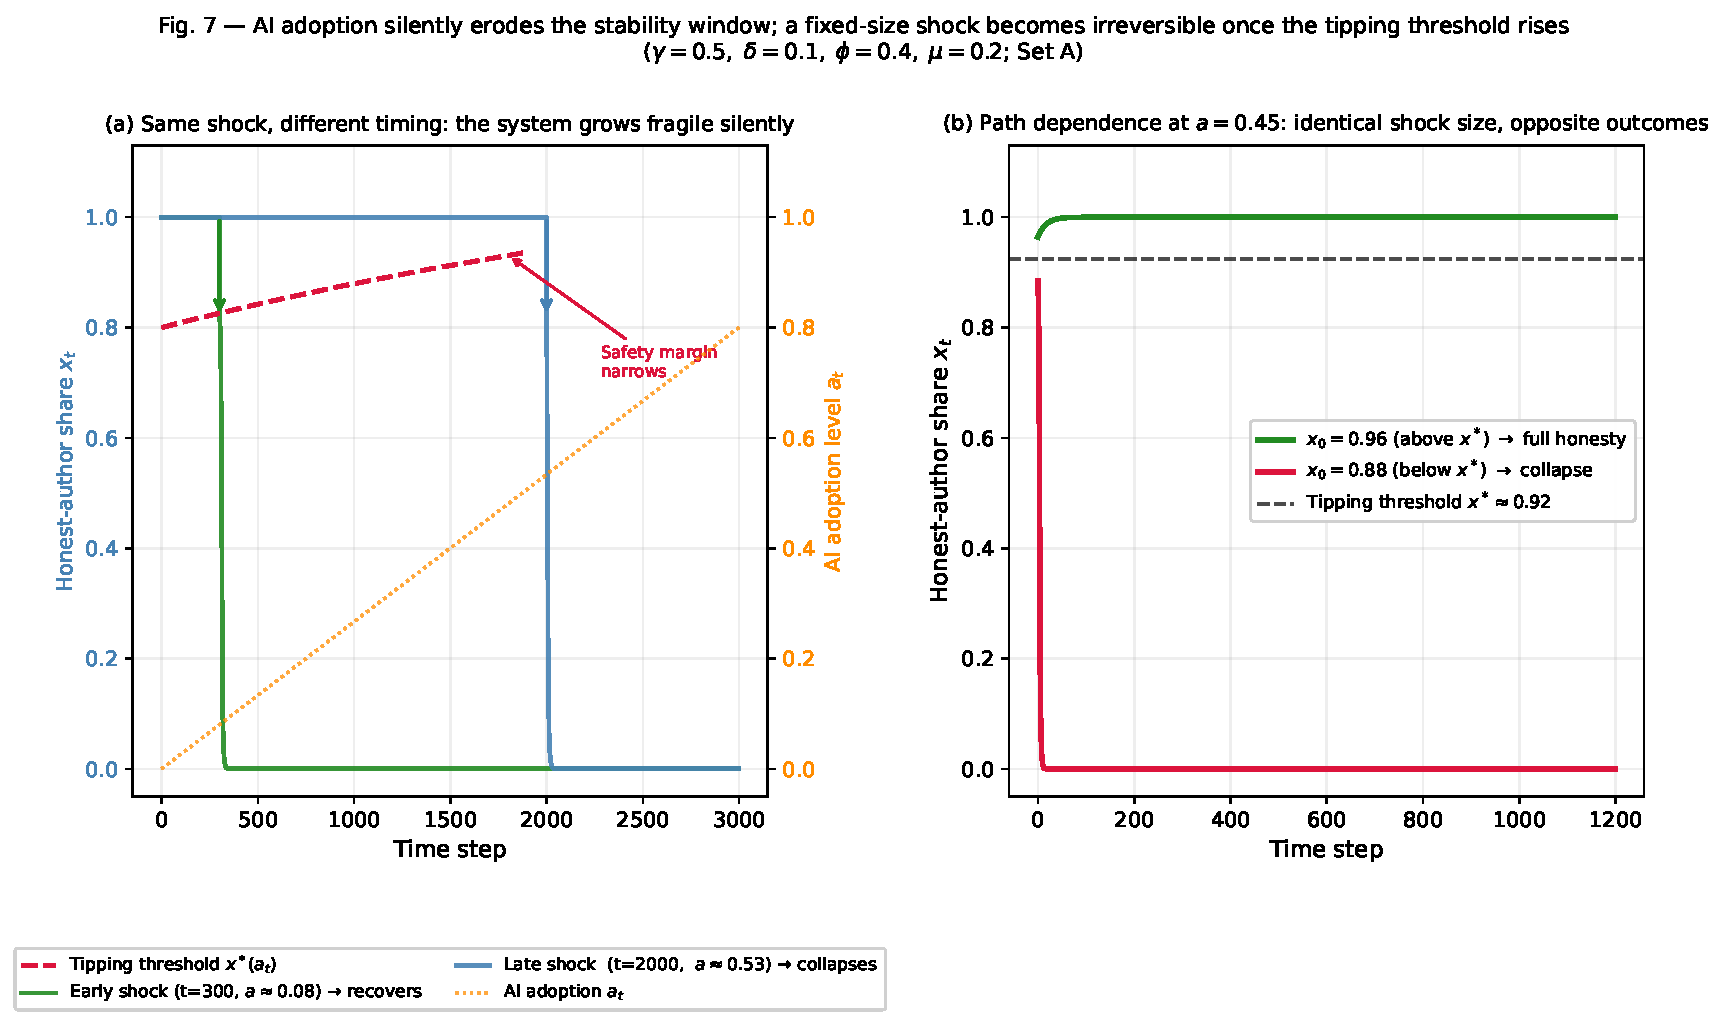
\includegraphics[width=\textwidth]{fig7_tipping_timeseries.pdf}
    \caption{\textbf{AI adoption silently erodes the stability window.}
    \textbf{(a)} The tipping threshold $x^*(a_t)$ (red dashed) rises monotonically from $\approx 0.80$ toward $x=1$ as $a$ increases through the bistability zone; the threshold ceases to exist above $a^* \approx 0.50$ (Set~A, analytical), when the system enters Global Corruption.
    A fixed-size shock of $\Delta x = 0.18$ recovers when applied at $a \approx 0.08$ (green; safety margin intact) but causes permanent collapse when applied at $a \approx 0.53$ (blue; system in GC, no stable honest long-run outcome).
    Observable quality gives no warning: $x_t \approx 1$ in both cases until the shock hits.
    \textbf{(b)} Path dependence at $a = 0.45$ (bistable zone, just below $a^*$): two initial conditions separated by $\Delta x_0 = 0.08$ diverge to opposite long-run outcomes, with the threshold near $x^*(0.45) \approx 0.92$.
    Parameters: Set~A, $\gamma=0.5$, $\delta=0.1$, $\phi=0.4$, $\mu=0.2$.}
    \label{fig:tipping_timeseries}
\end{figure}


\section{Robustness and Stochastic Validation}
\label{app:robustness}

\subsection{Robustness: Varying $\delta/\gamma$ and $\mu$}

Figure~\ref{fig:heatmap_outcomes} maps the long-run outcome across the two policy-sensitive dimensions identified in the analysis: the verification elasticity ratio $\delta/\gamma$ and the false-positive slope $\mu$.
Both panels are evaluated at $a = 0.8$, representing sustained high AI adoption.

Panel~(a) shows the long-run honest-author share $x^*$ on a continuous colour scale.
The parameter space is dominated by the collapse region ($x^* \approx 0$, dark red); a stable-honesty zone ($x^* \approx 1$, dark green) exists only in the bottom-right corner, where $\delta/\gamma \gtrsim 0.5$ and $\mu \lesssim 0.08$ simultaneously.
Panel~(b) confirms this pattern in terms of regime classification.
The baseline calibration ($\delta/\gamma = 0.2$, $\mu = 0.2$, marked by white dotted lines) lies solidly inside the Global Corruption zone.
The Bistability region (yellow) is confined to a narrow band at $\mu \lesssim 0.09$, independent of $\delta/\gamma$.
The Stable Coexistence and Global Honesty regions are accessible only when both conditions hold jointly; satisfying one alone is insufficient.

Two findings from this robustness check are particularly important.
First, the $\mu$ dimension is the binding constraint: even if $\delta/\gamma = 1$ (review capacity scales perfectly with submission volume), the system remains in Global Corruption whenever $\mu > 0.09$.
No investment in review staffing can compensate for a screening process that cannot distinguish polished AI text from genuine contributions \citep{Checco2021, Liang2023detectors}.
Second, the boundary between BS and GC is nearly vertical in the right panel, meaning that raising $\delta/\gamma$ from 0.2 to 0.5 shifts the system from GC to BS (where recovery is at least possible) only if $\mu$ is already low.
This interaction confirms that the two policy levers---raising $K_{rev}$ and reducing $\lambda$---must be deployed together, not sequentially.

\begin{figure}[H]
    \centering
    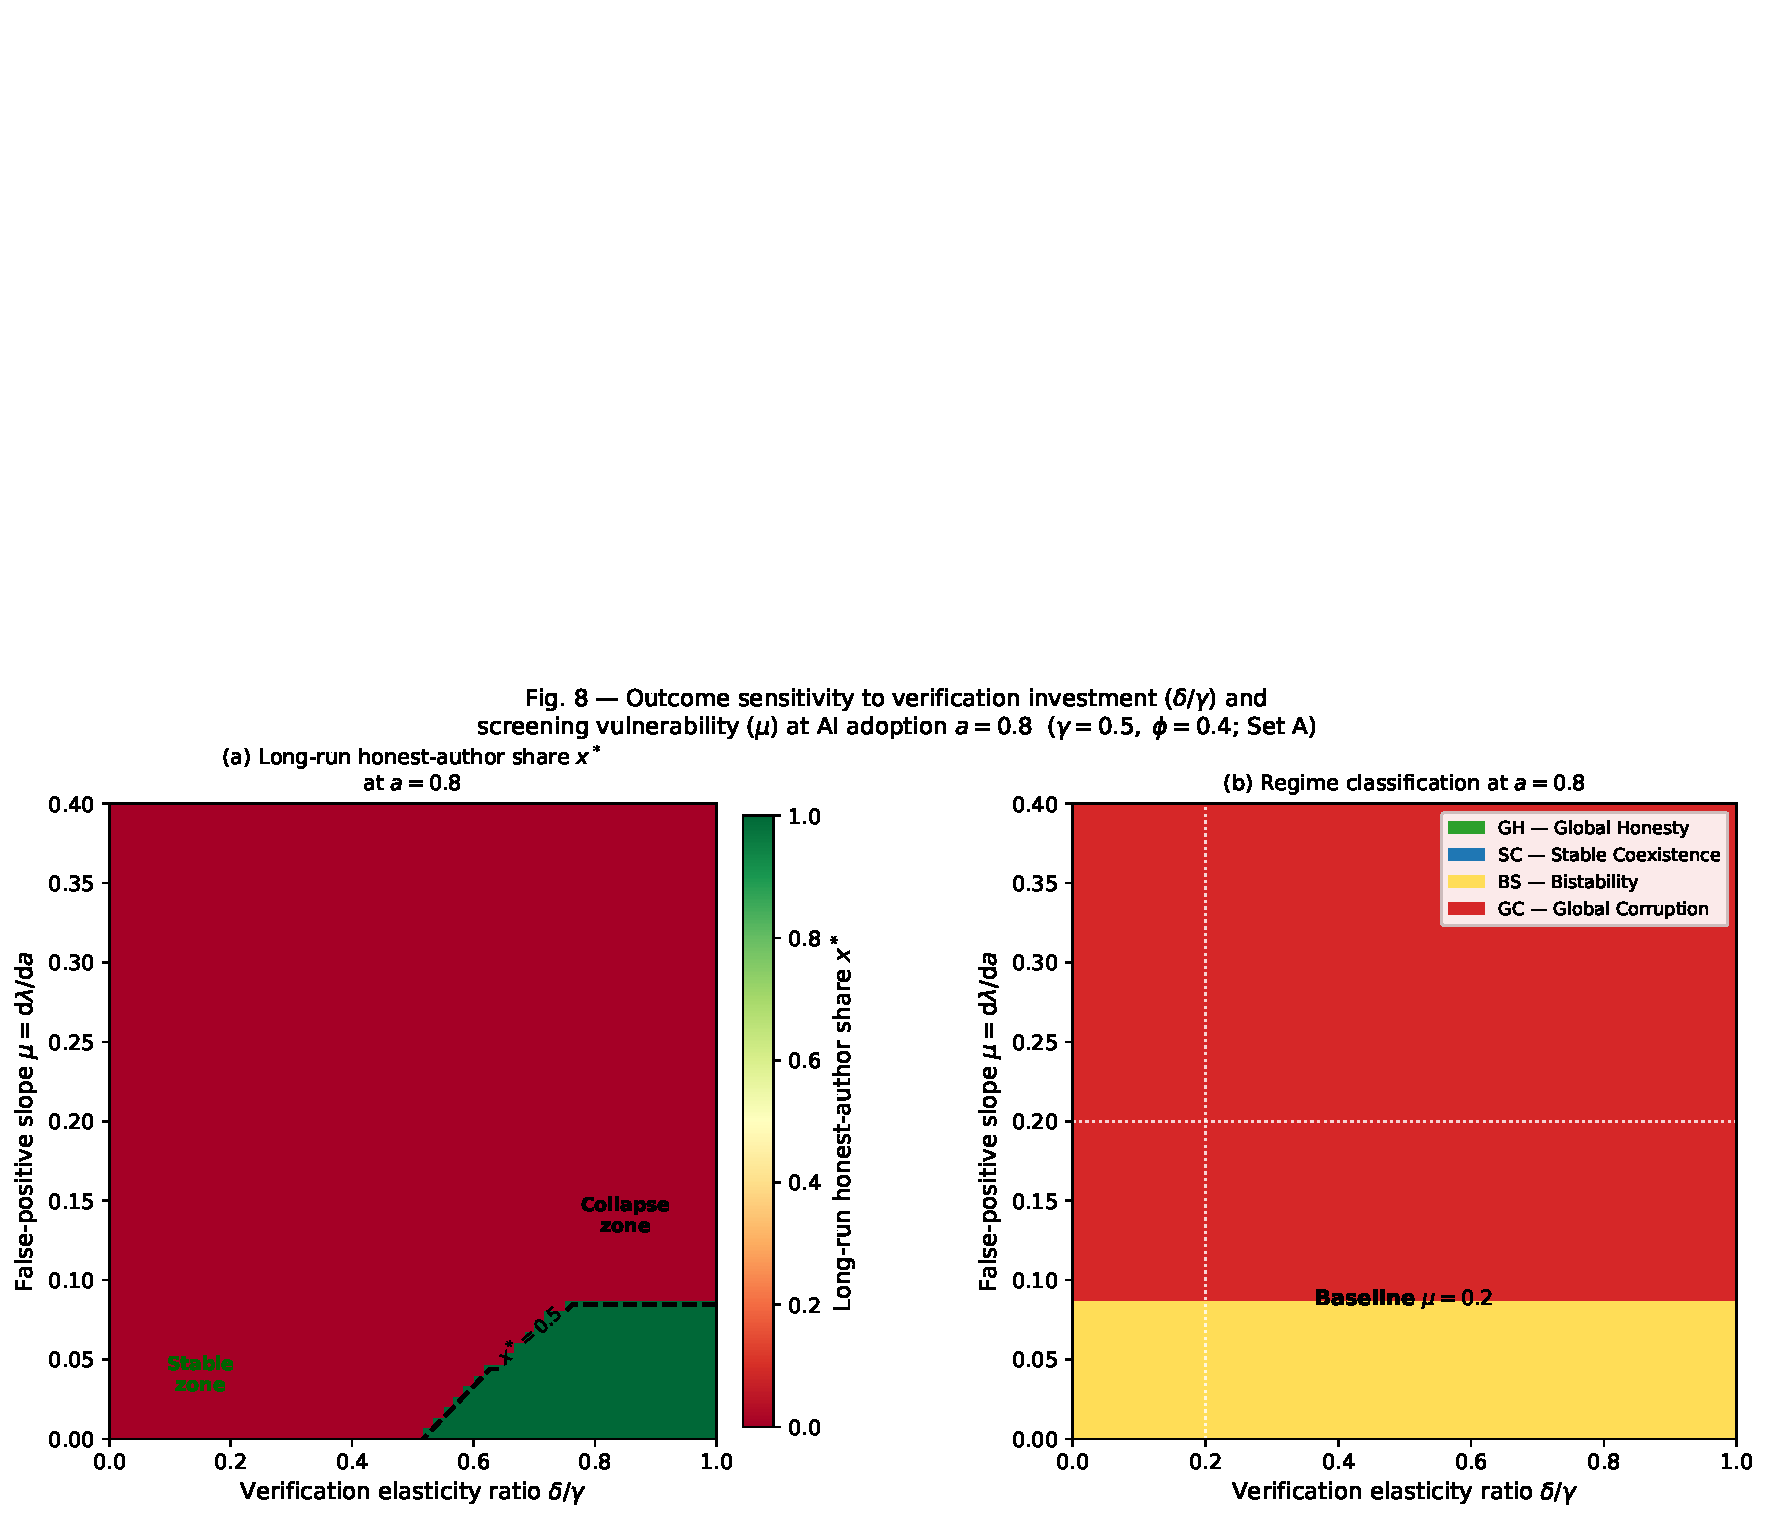
\includegraphics[width=\textwidth]{fig8_heatmap_outcomes.pdf}
    \caption{\textbf{Outcome sensitivity to verification investment and screening vulnerability.}
    Both panels are evaluated at $a = 0.8$ across a grid of $\delta/\gamma \in [0,1]$ and $\mu \in [0, 0.4]$.
    \textbf{(a)} Long-run honest-author share $x^*$: a stable-honesty zone (green) exists only when $\delta/\gamma \gtrsim 0.5$ and $\mu \lesssim 0.08$ simultaneously; the remainder of the space collapses ($x^* \approx 0$).
    \textbf{(b)} Regime classification: the baseline calibration (white dotted lines, $\delta/\gamma = 0.2$, $\mu = 0.2$) sits in Global Corruption.
    The Bistability corridor is narrow and confined to very low $\mu$.
    Global Honesty requires high $\delta/\gamma$ and low $\mu$ jointly.
    Parameters: $\gamma = 0.5$, $\phi = 0.4$; Set~A.}
    \label{fig:heatmap_outcomes}
\end{figure}

\subsection{Stochastic ABM: Does Finite-Population Noise Validate the ODE?}

The ODE assumes an infinitely large, well-mixed population and therefore suppresses all randomness.
Real academic communities are finite.
Even a system that sits nominally above the tipping threshold can cross it by chance when the number of authors is small \citep{Traulsen2009, Nowak2006}.
This subsection tests whether the deterministic tipping results survive under finite-population noise, and whether community size changes that verdict.

We extend the batch-matching ABM from \citet{Bonabeau2002} to incorporate the same rising AI adoption schedule ($a_t$ linear from 0 to 0.8 over 3{,}000 steps).
At each step $t$, the local screening capacity is $K_{rev,\text{eff}}(a_t) = K_{rev,0}\cdot(1+\delta a_t)/(1+\gamma a_t)$, the false-positive rate is $\lambda(a_t)$, the submission cost is $c(a_t)$, and the paper pool reaching the publication queue scales as $M(x,a_t)=(1+\gamma a_t)\cdot M_{\text{base}}(x,a_t)$---identical functional forms to the ODE\@.
The only departure from the ODE is that $N$ is finite and strategy revision is stochastic: each revision attempt uses the Fermi rule \citep{Szabo1998}, so the population does not move deterministically toward its expected next state but takes a noisy step.
To isolate pure demographic noise---the $1/\!\sqrt{N}$ fluctuations inherent to any finite population---we set batch size equal to $N$ in all conditions, so every agent participates in each round and no additional batch-level heterogeneity is introduced.
We run 100 independent replications for each of three community sizes---$N = 1{,}000$ (a large generalist field), $N = 500$ (a mid-size specialised field), and $N = 200$ (a small sub-field)---under two starting conditions that bracket the practical range of initial safety margins.
The \emph{margin scenario} starts at $x_0 = 0.82$, which is 0.02 above the initial tipping threshold $x^*(a=0) = 0.80$: a thin but nominally positive buffer.
The \emph{no-margin scenario} starts at $x_0 = x^*(0) = 0.80$, exactly at the tipping threshold, where the ODE's deterministic drift is zero and any noise can immediately push the system toward collapse.

Figure~\ref{fig:abm_validation} presents results across three panels.
Panel~(a) shows the margin scenario ($x_0 = 0.82$).
The ODE rises steadily toward $x \approx 1$: starting 0.02 above the tipping threshold, deterministic drift points toward full honesty.
All three ABM means track the ODE closely, converging to $x \approx 1$ within roughly 200 steps regardless of community size.
The 0.02 safety buffer is therefore universally protective: even the smallest community ($N = 200$) is not pushed below the threshold by demographic noise of order $1/\!\sqrt{N}$, because the buffer exceeds the typical fluctuation amplitude at all three population sizes tested.

Panel~(b) removes the buffer entirely ($x_0 = x^*(0) = 0.80$).
The ODE now declines toward $x \approx 0$: with no margin, deterministic drift immediately points downward as $a$ rises above zero.
The ABM tells a qualitatively different story.
All three community sizes decline sharply in the first 200--300 steps but then stabilise at an intermediate coexistence level---$N = 1{,}000$ near $x \approx 0.40$, $N = 500$ near $x \approx 0.47$, $N = 200$ near $x \approx 0.45$---well above the ODE's near-zero equilibrium.
This divergence reveals a structural limitation of the mean-field approximation: in a finite population, stochastic Fermi updating sustains a mixed-strategy steady state that the ODE cannot recover.
Community size has only a minor and non-monotone effect on the terminal level, confirming that population size is not the primary determinant of outcomes once the margin has been lost.

Panel~(c) quantifies both scenarios via collapse-fraction curves (collapse defined as $x < 0.3$, 100 replications).
In the margin scenario (solid lines), the collapse fraction is zero for all three community sizes across all adoption levels: no run crosses the collapse threshold, confirming that the 0.02 buffer is a robust shield regardless of $N$.
In the no-margin scenario (faded lines), the collapse fraction jumps to approximately $55$--$60\%$ at very low adoption levels ($a \approx 0.05$) and then plateaus.
The three $N$ values are tightly clustered throughout; $N = 1{,}000$ sits marginally above the smaller communities, consistent with larger populations converging more faithfully toward the ODE's lower equilibrium.

Three conclusions follow.
First, the safety margin $\Delta = x_0 - x^*(0)$ operates as an effective binary shield: a margin of even 0.02 prevents any collapse across all community sizes tested, while the complete absence of a margin exposes roughly half of all runs to quality decline irrespective of $N$.
Second, the ODE overestimates collapse severity when the margin is lost: finite-population stochasticity stabilises the system at a partial coexistence state ($x \approx 0.40$--$0.48$) rather than the ODE's near-zero long-run outcome, because Fermi noise sustains a residual share of honest authors that deterministic dynamics cannot maintain.
Third, community size is not a meaningful safeguard in either scenario: it neither rescues small fields when a margin exists (all recover regardless) nor provides meaningful protection when it does not (all decline to a similar partial-coexistence level).
Institutional design must therefore focus on actively maintaining a positive safety margin; community size alone cannot substitute for it.

\begin{figure}[H]
    \centering
    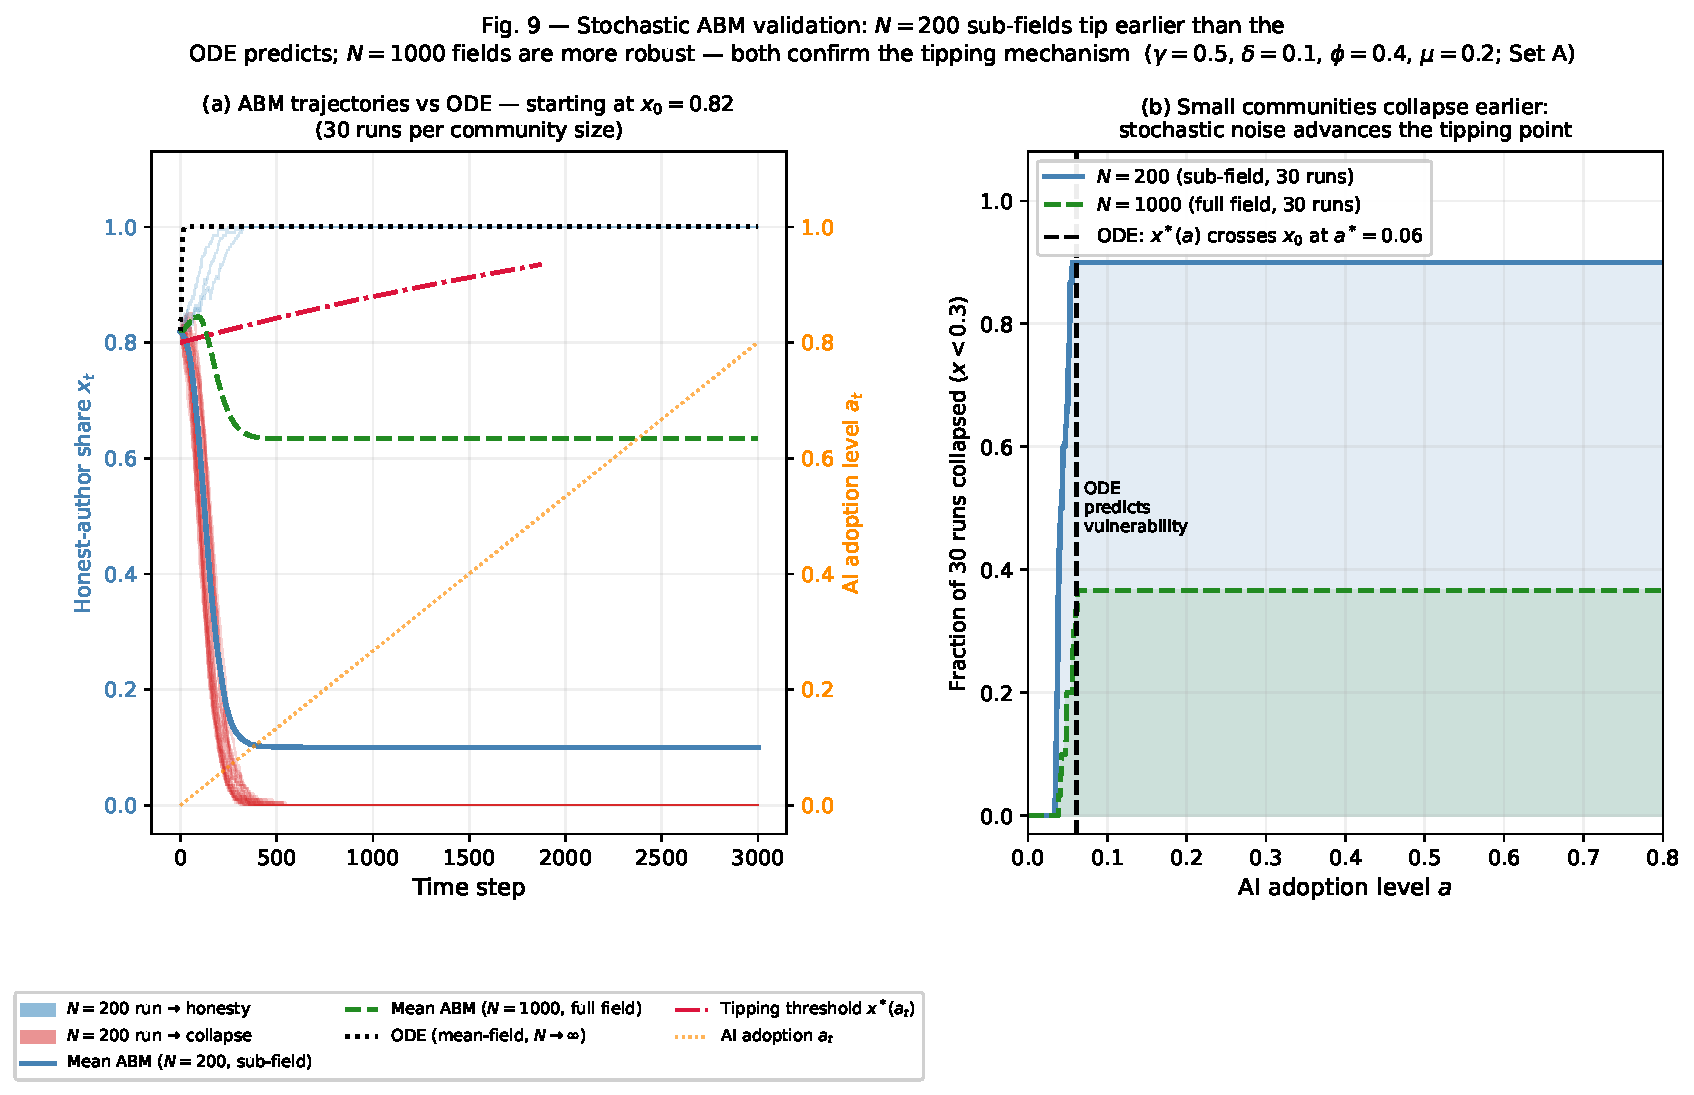
\includegraphics[width=\textwidth]{fig9_abm_validation.pdf}
    \caption{\textbf{Stochastic ABM vs ODE prediction.}
    All panels use Set~A parameters with a linear AI adoption ramp ($a_t$ from 0 to 0.8 over 3{,}000 steps) and batch size $= N$, isolating pure $1/\!\sqrt{N}$ demographic noise.
    \textbf{(a)} Mean ABM paths for $N \in \{200, 500, 1{,}000\}$ (100 replications each) vs the ODE, starting at $x_0 = 0.82$ (margin 0.02 above $x^*(0) = 0.80$).
    All ABM means and the ODE converge to $x \approx 1$; the 0.02 buffer is universally protective across all community sizes.
    \textbf{(b)} Same setup at $x_0 = 0.80$ (no margin).
    The ODE declines toward $x \approx 0$; all three ABM means decline sharply but stabilise at a stochastic coexistence state ($x \approx 0.40$--$0.48$), well above the mean-field prediction.
    \textbf{(c)} Collapse fraction ($x < 0.3$, 100 runs) as a function of $a$.
    Solid lines: margin scenario ($x_0 = 0.82$), zero collapse for all $N$ at all adoption levels.
    Faded lines: no-margin scenario ($x_0 = 0.80$), $\approx 55$--$60\%$ collapse fraction from $a \approx 0.05$, tightly clustered across $N$.
    Parameters: $\gamma=0.5$, $\delta=0.1$, $\phi=0.4$, $\mu=0.2$; Set~A.}
    \label{fig:abm_validation}
\end{figure}


\section{Welfare Analysis and Normative Policy Design}
\label{app:welfare}

\paragraph{Social welfare in a certification system.}
The publishing system produces two social goods beyond private author payoffs.
First, it generates \emph{scientific knowledge} as a public good: verified results can be used by downstream researchers, educators, practitioners, and policymakers at zero marginal cost, without depleting the original discovery \citep{DasguptaDavid1994}.
Second, it provides a \emph{certification signal}: a credential that allows readers to distinguish reliable findings from unreliable ones without re-examining every manuscript.
Degradation of this signal imposes social costs that no individual author internalises.
We define a reduced-form social welfare function:
\begin{equation}
  W(x,a) \;=\; \underbrace{N\bigl[x\,\Pi_{good}(x,a) + (1-x)\,\Pi_{bad}(x,a)\bigr]}_{\text{aggregate author surplus}}
  \;+\; \underbrace{S \cdot Q(x,a) \cdot \bar{M}(x,a)}_{\text{social value of certified knowledge}}
  \;-\; \underbrace{C(K_{rev})}_{\text{verification cost}},
  \label{eq:welfare}
\end{equation}
where $S > 0$ is the per-paper social value when quality is perfect, $Q(x,a) \equiv \alpha\pi_1 / [\alpha\pi_1 + (1-\alpha)(1-x)\pi_0/(x + (1-x))]$ is the precision of the certified pool (the fraction of accepted papers that are genuinely good), $\bar{M}(x,a)$ is total papers accepted per period, and $C(K_{rev})$ is the institutional cost of maintaining review capacity.
Welfare increases with $Q$ because a certified pool dominated by genuine contributions generates reliable knowledge cumulation, while $Q \approx 0$ produces noise that misdirects subsequent research and policy \citep{Ioannidis2005}.

\paragraph{The two externalities: why private and social incentives diverge.}
The individual spam payoff $\Pi_{bad}(x,a) = r\bar{\rho}\pi_0 - c$ omits two costs imposed on others.
The first is a \emph{congestion externality}.
When a spam author submits, total submission volume $V$ rises, which depresses screening intensity $\eta = \min(1, K_{rev}/V)$ and lowers the review quality received by every other submitter.
Peer-review attention is a finite shared resource, and individual overuse degrades the commons \citep{Ostrom1990}: each spam submission captures private value while imposing a diffuse cost on all other authors and editors.
The second is a \emph{certification externality}.
A low-quality paper, once accepted, reduces the precision $Q$ of the certified pool and degrades the informativeness of the certification signal for all downstream readers.
This is the quality-dilution mechanism in \citet{Akerlof1970}'s market for lemons: sellers of bad goods contaminate the quality signal, raising doubts about good goods and eroding the value of the entire market.
In academic publishing, the ``market'' is the pool of certified papers, the ``buyers'' are readers and downstream researchers, and ``bad goods'' are low-quality manuscripts that passed degraded peer review.
Neither externality is priced by the individual submitter.
The divergence between private and social returns is the canonical justification for corrective policy \citep{Pigou1920}.
Spamming is privately rational when $\Pi_{bad}(x,a) > 0$, but the full social cost includes the congestion externality imposed on honest authors and the certification-quality loss imposed on readers.
The socially optimal submission norm is therefore $x = 1$ (global honesty): this maximises $Q$, minimises wasteful review effort, and generates the highest social value from the certification pool.
Yet $x = 1$ is privately self-sustaining only when $\Pi_{bad}(1,a) < 0$; whenever AI adoption raises $\Pi_{bad}$ above zero, the social optimum and the private Nash equilibrium diverge.

\paragraph{Welfare ranking of the four regimes.}
Table~\ref{tab:welfare_regimes} ranks the four stable regimes by social welfare.
In GH ($x^* = 1$), no bad papers are submitted, the certified pool consists entirely of genuine work ($Q = 1$), and review resources are used efficiently.
In GC ($x^* = 0$), all authors submit bad papers alongside good ones, the certified pool is dominated by spam papers ($Q$ falls sharply under degraded screening), and the certification signal carries minimal information.
The welfare gap $\Delta W = W(1,a) - W(0,a) > 0$ is strictly positive even accounting for the higher author surpluses in GC, because the social-value term $S \cdot Q \cdot \bar{M}$ collapses in GC while the congestion cost of maintaining a large review apparatus to process a flood of mostly bad papers remains.
In SC ($x^* \in (0,1)$), welfare lies strictly between the two extremes.
In BS, expected welfare is a probability-weighted average of $W(1,a)$ and $W(0,a)$ determined by initial conditions and stochastic shocks: bistability is not itself a welfare outcome but a risk of tipping into GC from a currently-healthy GH state.

\begin{table}[H]
  \centering
  \footnotesize
  \caption{\textbf{Welfare ranking of the four stable regimes at a given AI adoption level $a$.}
    $Q^*$: precision of the certified pool (fraction of accepted papers that are genuine).
    $\eta^*$: screening intensity at the long-run equilibrium.
    Social welfare $W^*$ is the value of~\eqref{eq:welfare} evaluated at the long-run author composition $x^*$.}
  \label{tab:welfare_regimes}
  \setlength{\tabcolsep}{6pt}
  \begin{tabular}{lllllc}
    \toprule
    Regime & $x^*$ & $Q^*$ & $\eta^*$ & Author surplus & $W^*$ rank \\
    \midrule
    GH (Global Honesty)      & $1$          & High ($= 1$)          & High        & High (honest work rewarded)       & 1st (best)  \\
    SC (Stable Coexistence)  & $(0,1)$      & Medium                & Medium      & Mixed (both types coexist)        & 2nd         \\
    GC (Global Corruption)   & $0$          & Low ($\ll 1$)         & Low         & Positive (spam) but low social $S\cdot Q$ & 3rd  \\
    NS (No Submission)       & n/a          & n/a                   & n/a         & Zero                              & Dominated   \\
    \bottomrule
  \end{tabular}
\end{table}

\paragraph{Hysteresis amplifies the welfare loss.}
The welfare cost of AI adoption is not simply the static difference $W(1,a) - W(0,a)$; it is amplified by the hysteresis dynamic.
Once the system tips from GH into GC, restoring GH requires a large simultaneous intervention across $\lambda$, $K_{rev}$, and $c$.
This transition is costly: review infrastructure must be rebuilt, submission friction must be re-imposed, and reporting norms must be rehabilitated, all while the system is already in a low-quality long-run outcome that discourages investment in verification.
The ex-ante social cost of failing to prevent tipping therefore includes both the static welfare gap $\Delta W$ and the transition cost of recovery---a cost that is entirely avoided if preventive institutions are maintained \citep{Scheffer2001}.
This welfare-dynamic argument provides the theoretical foundation for the urgency of early intervention: the expected social benefit of preventing a tipping event is strictly larger than the expected benefit of correcting one after it occurs, because the correction requires additional resources and inflicts additional welfare losses during the recovery transition.

\paragraph{Normative policy recommendations.}
The welfare analysis converts the five institutional principles of the Institutional Responses section of the main text into a normative hierarchy ordered by welfare efficiency.
Four Corollaries follow from combining the welfare function~\eqref{eq:welfare} with Propositions 1--4.

\medskip
\noindent\textbf{Corollary W1 (Corrective levy on spam externalities).}
Because spam submissions impose unpriced negative externalities---congestion costs on honest authors and certification-quality losses on readers---the welfare-maximising policy imposes a corrective (Pigouvian) levy per submission equal to the marginal social cost of a spam attempt \citep{Pigou1920}.
In the model, this levy is equivalent to raising $c$: it restores the condition $c > r\lambda(a)$ that keeps GH stable, without restricting honest submissions if the levy is calibrated to the spam pass rate $\pi_0$ rather than applied uniformly.
Submission tokens and per-journal annual quotas are practical approximations of this levy: the normative case for them is not administrative convenience but welfare-theoretic---they correct a market failure, not merely a nuisance \citep{Cotton2013}.
An equity-preserving design issues token grants to authors at under-resourced institutions, ensuring that the levy targets strategic spamming rather than participation barriers.

\medskip
\noindent\textbf{Corollary W2 (Peer review as a public good requiring public funding).}
Peer review generates a public good: the certification signal is non-excludable (once published, the quality verdict is available to all readers) and the benefit of a thorough review is non-rival (every reader gains without diminishing others' access) \citep{DasguptaDavid1994}.
Private provision of public goods is sub-optimal under standard conditions: individual reviewers and journals do not capture the full social return from careful review, and competitive pressure to cut costs erodes voluntary supply below the socially efficient level.
The welfare-efficient remedy is public investment in $K_{rev}$---targeted grants for reviewer development programmes, structured-review recognition schemes, and journal subsidies for methods review---rather than relying on uncompensated voluntarism.
\citet{Aczel2021} propose transparent reviewer recognition systems as a coordination device that raises effective $K_{rev}$ without proportional budget increases; the normative case for mandating such systems is the public-good argument, not merely editorial preference.

\medskip
\noindent\textbf{Corollary W3 (Coordination mandate in the bistable region).}
Proposition~4 establishes that reducing $\lambda$ and raising $K_{rev}$ are unconditionally welfare-improving: they lower spam payoffs without harming honest authors.
However, decentralised adoption of verification standards is a coordination game with multiple equilibria: if competing journals do not adopt structured reporting requirements, rejected spam papers cycle to lower-tier venues, and no single journal captures the system-level benefit of its own investment in quality.
This cross-journal externality means the welfare-maximising outcome---universal verification standards---is not a Nash equilibrium of decentralised journal competition \citep{Ostrom1990}.
A mandatory field-wide standard, enforced by funders, accreditation bodies, or professional associations, internalises the cross-journal spillover and restores the welfare-efficient outcome.
The ClinicalTrials.gov registration mandate, which required prospective trial registration as a publication condition across many journals simultaneously, demonstrates that such coordination is institutionally feasible and welfare-improving even when no single journal would adopt the standard unilaterally \citep{Moher2009}.

\medskip
\noindent\textbf{Corollary W4 (Welfare ranking of institutional levers).}
The four levers of Proposition~4 have distinct welfare profiles.
First, reducing $\lambda$ (structured reporting, mandatory data sharing) is a \emph{Pareto improvement} relative to the unregulated equilibrium: it raises $Q^*$ and raises honest-author surplus by easing competition from spam, while imposing no direct cost on honest authors who already meet the new standard.
Second, raising $K_{rev}$ (public investment in review capacity) is welfare-improving when the congestion constraint is binding; it improves $Q^*$ and reduces the review burden per paper, with a cost borne by funders rather than authors.
Third, raising $c$ (Pigouvian levy) improves welfare when the spam externality cost exceeds the honest-author surplus loss from higher submission costs, which holds whenever $\Pi_{bad}(x,a) > 0$ and the honest-author share is substantial; the equity caveat is that the levy must be accompanied by targeted exemptions to avoid deterring genuine science.
Fourth, raising $K$ (expanding publication slots) is the \emph{unique lever that unconditionally reduces welfare}: it increases $\Pi_{bad}$ (Proposition~2), lowers $Q^*$ by attracting more spam, and degrades the certification signal for all readers, with no offsetting benefit.
The normative implication is unambiguous: expanding publication slot capacity without simultaneously reducing $\lambda$ is a welfare-reducing response to submission pressure, even though it appears to relieve editorial backlogs in the short run.
Backlogs are a symptom of submission congestion; expanding slots without fixing the underlying screening deficit treats the symptom while worsening the disease.

\begin{tcolorbox}[boxstyle, title={Box S1\quad Normative Policy Agenda: Welfare Priorities and Justifications}]
\small
\noindent\textbf{Welfare objective:}\;
Maximise $W(x,a) = \text{author surplus} + S \cdot Q \cdot \bar{M} - C(K_{rev})$ subject to the system converging to Global Honesty (GH), not Global Corruption (GC).

\medskip
\noindent\textbf{Market failures requiring correction:}
\begin{itemize}[noitemsep, topsep=2pt, leftmargin=*]
  \item \textit{Congestion externality}: each spam submission degrades review quality for all other authors by tightening $\eta = K_{rev}/V$.
  \item \textit{Certification externality}: each accepted spam paper dilutes the certified pool precision $Q$, reducing the value of certification for all readers (Akerlof lemons mechanism).
  \item \textit{Public-good underprovision}: peer review is non-rival and non-excludable; private voluntary supply is systematically below the socially optimal $K_{rev}$.
  \item \textit{Coordination failure}: no single journal internalises cross-journal quality spillovers; decentralised adoption of verification standards is sub-optimal.
\end{itemize}

\medskip
\noindent\textbf{Normative lever ranking (welfare-ordered):}

\smallskip
\noindent\begin{tabular}{@{}p{6.0cm}p{3.0cm}p{4.5cm}@{}}
Lever & Welfare effect & Normative justification \\
\midrule
$\lambda\downarrow$ (structured review, checklists, data sharing) & Pareto improvement & Corollary W1+W4; no side cost on honest authors \\
$K_{rev}\uparrow$ (public funding, recognition grants) & Welfare-improving & Corollary W2; public-good rationale \\
$c\uparrow$ (submission tokens, Pigouvian levy) & Welfare-improving$^*$ & Corollary W1; corrects congestion externality \\
Coordination mandate (field-wide standards) & Welfare-improving & Corollary W3; internalises cross-journal spillovers \\
$K\uparrow$ (more slots without $\lambda\downarrow$) & \textbf{Welfare-reducing} & Corollary W4; uniquely worsens certification quality \\
\end{tabular}

\smallskip
\noindent\footnotesize{$^*$ Subject to equity design: token grants for authors at under-resourced institutions.}

\medskip
\noindent\textbf{Priority sequencing:}
\begin{enumerate}[noitemsep, topsep=2pt, leftmargin=*]
  \item Deploy $\lambda\downarrow$ tools immediately: Pareto-improving and require no inter-journal coordination.
  \item Fund $K_{rev}\uparrow$ publicly: cannot be left to voluntary effort; public-good logic requires funder mandate.
  \item Implement Pigouvian $c\uparrow$ levy with equity exemptions: corrects the congestion externality.
  \item Mandate cross-journal coordination before tipping: welfare loss of coordination failure is preventable.
  \item Avoid $K\uparrow$ in isolation: any slot expansion must be paired with verified $\lambda\downarrow$ to prevent welfare deterioration.
\end{enumerate}

\medskip
\noindent\textit{Key welfare insight:}\;
The GH long-run outcome is both privately stable (when $\Pi_{bad} < 0$) and socially optimal.
The policy problem arises precisely when the private stability condition fails while the social optimum remains GH\@.
Welfare-efficient policy closes this gap by raising the private cost of spamming and the private return to honesty, not by expanding slots or ignoring the screening deficit.
\end{tcolorbox}


\section{Extended Empirical Predictions}
\label{app:predictions}

\paragraph{Prediction 3: Proxies for a rising false-positive rate.}
A rising $\lambda$ produces a detectable mismatch between surface quality and substantive reliability: manuscripts become more polished while methodological soundness does not improve proportionately.
Three observable proxies track this channel.
First, \textbf{acceptance rates} should rise faster than any improvement in underlying research quality, because easier-to-pass manuscripts inflate the acceptance pool without proportionate quality gains; \citet{Latona2024} document this experimentally---AI-assisted reviews award systematically higher scores.
Second, \textbf{surface linguistic quality} should improve independently of replication success or citation impact.
\citet{Kobak2025} show that AI modification is measurable through excess vocabulary, providing a continuous field-level proxy for surface polish that can be compared against downstream quality indicators.
Third, \textbf{replication rates} should decline in fields with high AI adoption if the screening signal is genuinely degrading.
The Open Science Collaboration found that fewer than half of 100 psychology studies replicated successfully \citep{OSC2015}; replicating that audit with papers published after 2022 in high-AI-adoption fields, and comparing against low-adoption fields, would directly test whether the false-positive channel is active.

\paragraph{Prediction 4: Proxies for review-capacity stress.}
The model predicts declining screening intensity $\eta = \min(1, K_{rev}/V)$ as submission volume grows faster than review capacity.
Four observable proxies track this channel.
First, \textbf{reviewer invitation acceptance rates} should decline faster in high-AI-adoption fields; \citet{Meyerson2025} document a continuous 21-year decline at a single journal, and the model predicts this trajectory steepens as AI-driven submission pressure intensifies.
Second, \textbf{editorial turnaround times} should lengthen as editors wait longer for reviewer responses, signalling scarcity in the review pool.
Third, \textbf{desk rejection rates} should rise as editorial offices pre-filter to protect reviewers from overload; an increasing share of submissions receiving no substantive evaluation is a direct proxy for $\eta$ falling toward zero for that fraction of papers.
Fourth, \textbf{reviewer concentration} should increase---a growing Gini coefficient on review counts across the active reviewer pool indicates that a shrinking fraction of researchers is absorbing a rising fraction of the total burden, a pattern that preceded the current shortage \citep{Kovanis2016}.

\paragraph{Prediction 5: Data sources and identification strategy.}
Testing these predictions requires field-level panel data on both the production and verification sides of the system.
Several existing sources can be combined.
On the production side, arXiv submission records are public, monthly, and tagged by subfield; the LLM modification classifier of \citet{Liang2025}, applied to these records, provides a continuous field-level estimate of $a_t$.
The vocabulary-based detection approach of \citet{Kobak2025}, applied across the 15-million-abstract PubMed archive, offers an independent measure of AI modification at the sub-discipline level.
On the verification side, reviewer acceptance rate series can be constructed from editorial logs at journals that publish annual statistics; acceptance rates, turnaround times, and retraction counts are available at scale through OpenAlex, CrossRef, and the Retraction Watch database.
The natural experiment for causal identification is the release of ChatGPT in November 2022, which created a sharp and field-heterogeneous shock to submission cost $c$.
A difference-in-differences design would compare fields with high ex-ante AI amenability---measured by pre-2022 adoption of computational tools, large collaborative networks, or text-heavy output---against low-amenability fields, before and after November 2022.
The prediction is that high-amenability fields show faster growth in submission-to-review ratios, rising acceptance rates, and more rapid accumulation of post-publication retractions relative to low-amenability fields, controlling for field size and pre-shock submission trends.

\paragraph{Prediction 6: What would falsify the asymmetry hypothesis.}
The model's conclusions rest on two empirical claims: production scales faster than verification ($\gamma > \delta$), and the false-positive rate rises with AI adoption ($\mu > 0$).
Either claim failing empirically would revise the institutional implications.
If $\delta \approx \gamma$---if AI-assisted reviewing tools raise review capacity at nearly the same rate as AI raises submission volume---the congestion channel would not activate.
This would be observable as stable submission-to-acceptance ratios and constant turnaround times despite rising submission volumes in high-adoption fields.
If $\mu \approx 0$---if AI tools improve screening reliability, perhaps because structured AI-assisted checklists close the gap that polished writing opens---the false-positive channel would be neutralised.
This would be observable as stable or falling acceptance rates in high-AI-adoption fields combined with stable replication rates for newly published work.
The robustness analysis in Figure~\ref{fig:heatmap_outcomes} shows that $\mu$ is the binding parameter: even if $\delta/\gamma$ rises toward 1, the system remains in Global Corruption whenever $\mu > 0.09$.
A finding that AI-assisted reviewing consistently \emph{improves} score calibration---rather than inflating it---would therefore be the strongest possible disconfirmation of the model's policy conclusions \citep{Checco2021}.
The available evidence currently points in the opposite direction \citep{Latona2024, Liang2024ICML, Naddaf2025}.


\section{Model Extensions}
\label{app:extensions}

\paragraph{AI adoption as a scalar: limits and heterogeneity.}
We represent AI adoption with a single scalar $a$ that aggregates the fraction of authors using AI tools and the intensity of their use.
This captures the mean effect but suppresses two empirically important dimensions.
The first is task heterogeneity.
AI excels at drafting and reformatting text but falls short of replicating the judgment required for novel empirical analysis \citep{Checco2021}.
The production elasticity $\gamma$ therefore measures AI's effect on submission volume rather than on genuine scientific output.
A model that separates writing assistance from research assistance would generate sharper predictions about $\mu$: fields where AI mainly improves surface fluency face a higher $\mu$ than fields where AI genuinely improves research quality.
The second dimension is cross-author heterogeneity in adoption timing.
Early adopters gain a first-mover advantage under current publication incentives, and social learning then accelerates diffusion through the same imitation dynamics documented for other general-purpose technologies \citep{Rogers2003}.
As shown in Appendix~\ref{app:abm}, stochastic fluctuations from a concentrated wave of intensive early adopters can push a finite community below its tipping threshold before field-wide mean adoption reaches a critical level.
Heterogeneous adoption therefore makes tipping events more likely and less predictable than the scalar analysis implies.

\paragraph{Multi-journal competition and quality cascades.}
Extending the model to a hierarchy of competing journals would capture dynamics absent from our analysis.
When authors face multiple venues, rejection does not dissipate submission pressure---it routes it to the next tier.
\citet{Clauset2015} document steep and persistent prestige hierarchies in academic hiring networks; analogous hierarchies characterise journals, where a small number of high-impact venues confer disproportionate career rewards $r$.
In a tiered model, the slot expansion paradox would have a cross-venue counterpart: entry of new low-tier journals raises total certification capacity $K$ without improving screening quality $\lambda$, raising $\Pi_{bad}$ at every tier simultaneously.
\citet{Zollman2024} show that prestige-maximising incentives in multi-journal settings already reward strategic over honest behaviour; AI adoption amplifies this dynamic by lowering $c(a)$ and raising $\lambda(a)$ for the entire author population.
The institutional implication is that verification standards must be coordinated across journal tiers.
A single journal raising $K_{rev}$ and lowering $\lambda$ provides limited system-level protection if rejected spam papers are absorbed by lower-tier venues and ultimately circulate as certified work.
Overlay certification models---where a shared preprint layer is evaluated by tier-specific panels with explicit quality standards---are one architecture that could enforce coordination without requiring every journal to act simultaneously.

\paragraph{Endogenous rewards, reviewer effort, and reputation systems.}
Two parameters we treat as fixed---the publication reward $r$ and the reviewer participation rate embedded in $K_{rev}$---are endogenous to institutional design, and relaxing this assumption would enrich the model.
On the reward side, $r$ reflects career-level incentives to publish.
Evaluation frameworks that weight publication counts heavily inflate $r$ for marginal submissions; shifting toward impact-based or reproducibility-weighted assessment directly reduces $r$ and shrinks the parameter region where $\Pi_{bad} > 0$ \citep{Hicks2015}.
\citet{Stephan2012} traces publication inflation to career structures that treat paper counts as a proxy for scientific value; AI adoption compounds this pre-existing incentive problem by making low-quality output cheaper to produce.
On the reviewer side, we model $K_{rev}$ as a hard capacity constraint, but reviewer effort per paper is also a margin.
Reviewer participation has declined continuously for two decades \citep{Meyerson2025}, and the decline accelerates if quality collapse erodes the perceived value of certification---a positive feedback loop that our model does not capture.
An extension treating reviewer effort as endogenous would predict that transparency mechanisms---publishing review reports, providing structured evaluation templates, recognising reviewer contributions \citep{Aczel2021}---can raise effective screening accuracy without increasing the number of reviewers.
The two levers---more reviewers and better effort per reviewer---address the same capacity constraint $K_{rev}$ through different margins and should be designed jointly.
Neither is sufficient in isolation when $\lambda > c(a)/r$, the binding condition identified in the main text.


\section{Model Summary, Reference Tables, and Policy Boxes}
\label{app:reference}

This appendix collects the summary boxes and reference tables from the main text, providing compact overviews of the baseline model, AI extension, parameter calibration, and institutional policy menu.

\begin{tcolorbox}[boxstyle, title={Box S2\quad The Baseline Model in Brief}]
\small
\textbf{Parameters.}\;
$N$: author population;\;
$\alpha$: probability a paper is genuinely good;\;
$x$: share of selective (OG) authors;\;
$K_{rev}$: review capacity;\;
$K$: publication slots;\;
$r$: publication reward;\;
$c$: submission cost;\;
$\lambda$: false-positive rate (bad paper passes review);\;
$\varepsilon$: false-negative rate (good paper rejected).

\medskip
\textbf{Two bottlenecks.}\;
Submission volume $V(x)=N[1-(1-\alpha)x]$ rises as the always-submit (AS) share grows.
\[
  \eta(x)=\min\!\left(1,\tfrac{K_{rev}}{V(x)}\right)
  \quad\text{screening intensity --- falls below 1 when volume exceeds capacity, diluting scrutiny per paper}
\]
\[
  \bar{\rho}(x)=\min\!\left(1,\tfrac{K}{M(x)}\right)
  \quad\text{rationing probability --- falls below 1 when accepted papers exceed slots}
\]
where $M(x)=N\alpha\,\pi_1(x)+N(1-\alpha)(1-x)\,\pi_0(x)$ is the peer-accepted pool.

\medskip
\textbf{Pass rates under congestion.}
\begin{align*}
  \pi_0(x)&=1-\eta(x)(1-\lambda) &\text{bad paper passes; rises as scrutiny is diluted}\\
  \pi_1(x)&=1-\eta(x)\,\varepsilon &\text{good paper passes; rises as scrutiny is diluted}
\end{align*}

\textbf{Spam payoff and dynamics.}
\[
  \Pi_{bad}(x)=r\cdot\bar{\rho}(x)\cdot\pi_0(x)-c
  \qquad\Longrightarrow\qquad
  \dot{x}=-x(1-x)(1-\alpha)\,\Pi_{bad}(x)
\]
$\Pi_{bad}>0$: AS spreads, $x$ falls.\quad $\Pi_{bad}<0$: OG spreads, $x$ rises.

\medskip
\textbf{Four long-run outcomes} (determined by the signs of $\Pi_{bad}$ at the two boundaries):\smallskip

\noindent
\begin{tabular}{@{}llll@{}}
\toprule
Regime & $\Pi_{bad}(1)$ & $\Pi_{bad}(0)$ & Long-run outcome \\
\midrule
\textbf{GH} & $<0$ & $<0$ & $x=1$: all authors submit only good work \\
\textbf{GC} & $>0$ & $>0$ & $x=0$: all authors submit regardless of quality \\
\textbf{BS} & $<0$ & $>0$ & Both $x=1$ and $x=0$ stable; history decides \\
\textbf{SC} & $>0$ & $<0$ & Interior $x^*$; slot rationing deters spam \\
\bottomrule
\end{tabular}

\smallskip
\textit{Key insight:} The honest boundary ($x=1$) is secured by keeping $\lambda$ low.
The corrupt boundary ($x=0$) is held by keeping $K$ tight.
The two bottlenecks can therefore be targeted \emph{separately} as policy instruments.
\end{tcolorbox}


\begin{table}[H]
\centering
\caption{\textbf{AI adoption channels and their model counterparts.}
Each row maps an empirical mechanism to the corresponding model parameter,
the direction of the shift, and the evidence base.}
\label{tab:ai_channels}
\renewcommand{\arraystretch}{1.4}
\begin{tabularx}{\textwidth}{p{2.8cm} p{4.0cm} c c p{3.6cm}}
\toprule
\textbf{Empirical channel} & \textbf{Mechanism} & \textbf{Parameter} & \textbf{Shift} & \textbf{Key evidence} \\
\midrule
Lower drafting cost
  & AI reduces time and effort per manuscript; resubmission friction falls
  & $c(a)$
  & $\downarrow$
  & \citet{NoyZhang2023}; \citet{StokelWalker2023} \\
Higher submission volume
  & More authors submit more frequently; low-quality papers enter the pool
  & $V$ (elasticity $\gamma$)
  & $\uparrow$
  & \citet{arXiv2024}; \citet{Liang2025}; \citet{Kobak2025} \\
Lagging review capacity
  & Deep verification remains human-intensive; policy restricts AI in review; reviewer shortage pre-dates AI
  & $K_{rev}$ (elasticity $\delta < \gamma$)
  & $\uparrow$ slowly
  & \citet{Meyerson2025}; \citet{Kovanis2016}; \citet{Naddaf2025} \\
Rising false-positive rate
  & Polished AI text harder to distinguish; AI-assisted reviews inflate acceptance scores; detectors unreliable
  & $\lambda(a)$
  & $\uparrow$
  & \citet{Liang2024ICML}; \citet{Latona2024}; \citet{Liang2023detectors} \\
Possible quality uplift
  & AI may also help authors improve genuine contributions (partial offset)
  & $\alpha$
  & $\uparrow$ (offset)
  & \citet{NoyZhang2023} \\
\bottomrule
\end{tabularx}
\end{table}


\begin{tcolorbox}[boxstyle, title={Box S3\quad What AI Changes: Parameter Shifts and the Asymmetry}]
\small
\textbf{AI adoption parameter.}\;
$a\in[0,1]$: field-level AI adoption intensity ($a=0$ = pre-AI baseline; $a=1$ = full adoption).

\medskip
\textbf{Four channels and their functional forms.}\smallskip

\noindent
\begin{tabular}{@{}p{3.2cm}p{7.0cm}cl@{}}
\toprule
Channel & Functional form & Direction & Key parameter \\
\midrule
Submission volume    & $V(x,a)=N[1-(1-\alpha)x]\cdot(1+\gamma a)$ & $\uparrow$ & elasticity $\gamma$ \\
Submission cost      & $c(a)=c_0(1-\phi\, a)$                      & $\downarrow$ & slope $\phi\in(0,1)$ \\
False-positive rate  & $\lambda(a)=\lambda_0+\mu\, a$              & $\uparrow$ & slope $\mu\geq 0$ \\
Review capacity      & $K_{rev}(a)=K_{rev}(0)\cdot(1+\delta\, a)$  & $\uparrow$ slowly & elasticity $\delta<\gamma$ \\
\bottomrule
\end{tabular}

\medskip
\textbf{The asymmetry assumption:}\; $\gamma>\delta\geq 0$ --- production scales faster than verification.

\medskip
\textbf{Net effect on spam payoff.}
\[
  \frac{\partial\Pi_{bad}(x,a)}{\partial a}
  \;=\;\underbrace{r\mu}_{{\lambda\uparrow}}
  \;+\;\underbrace{c_0\phi}_{c\downarrow}
  \;+\;\underbrace{[\text{congestion terms}]}_{>0\text{ when }\gamma>\delta}
  \;>\;0
  \qquad\text{for all }x\in(0,1).
\]
AI makes submitting low-quality work more attractive at \emph{every} composition of the author population.

\medskip
\textbf{Closed-form tipping threshold} (honest boundary $x=1$, uncongested case):
\[
  a^{*}=\frac{c_0-r\lambda_0}{r\mu+c_0\phi}.
\]
Above $a^{*}$, $\Pi_{bad}(1,a)>0$: the honest long-run outcome is no longer self-sustaining.
For Set~A parameters: $a^{*}=(25-10)/(20+10)=0.50$.

\medskip
\textit{Key insight:}\; $a$ is largely exogenous, but $\delta$ (verification investment) and $\mu$ (screening vulnerability) are policy choices.
\end{tcolorbox}


\begin{table}[hbt!]
\centering
\caption{\textbf{Scenario matrix: qualitative regime outcomes as AI adoption $a$ rises.}
Two policy-sensitive parameters determine the trajectory.
$\delta/\gamma$: how fast review capacity keeps pace with submission volume (a measure of investment in verification infrastructure).
$\mu$: how fast AI adoption raises the false-positive rate (a measure of screening vulnerability).
Each cell describes the dominant direction of regime change as $a$ increases from zero.}
\label{tab:scenario_matrix}
\renewcommand{\arraystretch}{1.6}
\small
\begin{tabularx}{\textwidth}{p{3.0cm} X X}
\toprule
 & \textbf{$\delta \approx \gamma$: review keeps pace} & \textbf{$\delta \ll \gamma$: review lags severely} \\
\midrule
\textbf{$\mu > 0$:} screening degrades
  & \textit{Partial stability.}
    Review congestion is controlled, but rising $\lambda$ still weakens the screening signal.
    GH region shrinks; bistability expands.
    Verification investment is necessary but not sufficient.
  & \textit{Highest risk.}
    Both the congestion and false-positive channels are active.
    $\Pi_{bad}(1,a)$ rises rapidly.
    The system moves toward Global Corruption.
    Risk of irreversible tipping is high. \\
\midrule
\textbf{$\mu \approx 0$:} screening holds
  & \textit{Stable.}
    AI raises both production and verification at comparable rates; screening quality is maintained.
    GH region is preserved.
    Consistent with AI-augmented structured review under strong institutional controls.
  & \textit{Conditionally stable.}
    Slot rationing may still provide defence by congestion if $K$ is tight.
    Fragile: any expansion of publication slots or rise in $r$ can tip the system toward bistability.
    Requires active management of $K$. \\
\bottomrule
\end{tabularx}
\end{table}


\begin{table}[hbt!]
    \centering
    \caption{\textbf{Parameter calibration for numerical analysis.}}
    \label{tab:calibration}
    \renewcommand{\arraystretch}{1.2}
    \begin{tabular}{clcc}
        \toprule
        \textbf{Symbol} & \textbf{Description} & \textbf{Set A (Baseline)} & \textbf{Set B (Top-tier)} \\
        \midrule
        $N$          & Author population       & 1000          & 1000 \\
        $\alpha$     & Good-paper probability  & 0.2           & 0.2  \\
        \midrule
        $K_{rev}$    & Review capacity         & \textbf{300}  & \textbf{1200} \\
        $K$          & Slot capacity           & \textbf{400}  & \textbf{180}  \\
        \midrule
        $r$          & Publication reward      & 100           & \textbf{150}  \\
        $c$          & Submission cost         & 25            & \textbf{30}   \\
        $\lambda$    & False-positive rate     & 0.1           & \textbf{0.4}  \\
        $\varepsilon$& False-negative rate     & 0.05          & 0.01          \\
        \bottomrule
    \end{tabular}
    \smallskip\\
    \footnotesize{\textit{Set~A: review bottleneck dominates; primary failure mode is bistability.
    Set~B: slot scarcity dominates; illustrates defence by congestion.}}
\end{table}


\begin{table}[H]
  \centering
  \footnotesize
  \caption{\textbf{Institutional mechanisms and their model parameter effects.}
    Each row maps a concrete institution to the parameter it primarily shifts.
    Arrows: $\uparrow$ raises, $\downarrow$ lowers, \textemdash\ no direct effect, $\uparrow\!(\cdot)$ / $\downarrow\!(\cdot)$ partial or indirect effect.
    Principle~5 operates on a longer horizon than Principles~1--4 and requires coordination across funders and institutions.}
  \label{tab:institutions}
  \setlength{\tabcolsep}{4pt}
  \resizebox{\textwidth}{!}{%
  \begin{tabular}{p{3.8cm}p{3.4cm}cccccp{1.3cm}}
    \toprule
    Institution & Mechanism summary & $K_{rev}$ & $\lambda$ & $c$ & $r$ & $K$ & Horizon \\
    \midrule
    \multicolumn{8}{l}{\textit{Principle 1: Scale verification}} \\
    \addlinespace
    Structured reviewer panels \& recognition      & Reward and recognise review effort           & $\uparrow$        & \textemdash & \textemdash & \textemdash & \textemdash & Quick  \\
    AI-assisted pre-screening (format/consistency) & Flag obvious flaws before expert review      & $\uparrow$        & \textemdash & \textemdash & \textemdash & \textemdash & Quick  \\
    \midrule
    \multicolumn{8}{l}{\textit{Principle 2: Reduce false-positive rate}} \\
    \addlinespace
    Mandatory data, code, and materials sharing    & Enables post-submission verification         & $\uparrow(\cdot)$ & $\downarrow$          & $\uparrow(\cdot)$ & \textemdash & \textemdash & Quick  \\
    Structured reporting checklists (CONSORT/PRISMA) & Forces method transparency               & \textemdash       & $\downarrow$          & \textemdash       & \textemdash & \textemdash & Quick  \\
    Registered Reports (pre-registered design)     & Eliminates outcome-selective reporting       & $\uparrow(\cdot)$ & $\downarrow\downarrow$ & $\uparrow$        & \textemdash & \textemdash & Medium \\
    Dedicated statistical/methods editorial review & Specialist check of analytic choices         & $\uparrow$        & $\downarrow$          & \textemdash       & \textemdash & \textemdash & Quick  \\
    \midrule
    \multicolumn{8}{l}{\textit{Principle 3: Add smart friction}} \\
    \addlinespace
    Annual submission tokens or quotas             & Raise cost of marginal submissions           & \textemdash & \textemdash & $\uparrow\uparrow$ & \textemdash & \textemdash & Quick  \\
    Escalating resubmission fees                   & Target low-cost paper cycling                & \textemdash & \textemdash & $\uparrow$         & \textemdash & \textemdash & Quick  \\
    Pre-submission triage/desk-rejection filter    & Reject obvious mismatches before review      & $\uparrow(\cdot)$ & $\downarrow(\cdot)$ & \textemdash & \textemdash & \textemdash & Quick  \\
    \midrule
    \multicolumn{8}{l}{\textit{Principle 4: Decouple dissemination}} \\
    \addlinespace
    Preprint $+$ overlay certification layer       & Separate speed from quality guarantee        & $\uparrow$ & \textemdash & \textemdash & \textemdash & $\downarrow$ (cert.) & Deep \\
    \midrule
    \multicolumn{8}{l}{\textit{Principle 5: Reshape evaluation rewards}} \\
    \addlinespace
    Impact-weighted / reproducibility-indexed assessment & Reduce $r$ for marginal output; raise $r$ for replication and quality & \textemdash & \textemdash & \textemdash & $\downarrow$ & \textemdash & Deep \\
    \midrule
    \multicolumn{8}{l}{\textit{Transition: post-collapse reset}} \\
    \addlinespace
    Coordinated field-wide mandate                 & Simultaneous cross-journal reform push       & $\uparrow\uparrow$ & $\downarrow\downarrow$ & $\uparrow\uparrow$ & \textemdash & \textemdash & Crisis \\
    \bottomrule
  \end{tabular}}
\end{table}


\begin{tcolorbox}[boxstyle, title={Box S4\quad Policy Menu: Institutions, Levers, and Sequencing}]
\small
\textbf{Goal.}\;
Keep $\Pi_{bad}(x,a)<0$ as AI adoption $a$ deepens.
\textbf{Binding constraint:}\; $\lambda(a)<c(a)/r$ --- when violated, no increase in $K_{rev}$ alone can restore Global Honesty.

\medskip
\noindent\textit{Quick wins} (no inter-journal coordination required):\smallskip

\noindent
\begin{tabular}{@{}p{8.2cm}l@{}}
Structured reporting checklists (CONSORT, PRISMA) & $\lambda\downarrow$ \\
Mandatory data and code sharing                   & $\lambda\downarrow$,\;$c\uparrow$ (partial) \\
Submission token caps / annual per-journal quotas & $c\uparrow\uparrow$ \\
Escalating resubmission fees                      & $c\uparrow$ \\
AI-assisted format and consistency pre-screening  & $K_{rev}\uparrow$ \\
\end{tabular}

\medskip
\noindent\textit{Deep redesign} (requires collective action across journals or fields):\smallskip

\noindent
\begin{tabular}{@{}p{8.2cm}l@{}}
Preprint servers + overlay certification layer         & decouple dissemination from $K_{cert}$ \\
Cross-journal quota systems                           & $c\uparrow$ system-wide \\
Coordinated field-wide mandate                        & $K_{rev}\uparrow\uparrow$,\;$\lambda\downarrow\downarrow$,\;$c\uparrow\uparrow$ \\
\end{tabular}

\medskip
\noindent\textit{After tipping} (recovery, not prevention):\;
Once in Global Corruption ($\Pi_{bad}>0$ everywhere), only a \emph{large, simultaneous} intervention across $K_{rev}$, $\lambda$, and $c$ can shift the system out of the GC region.
Gradual, journal-by-journal reform is insufficient.

\medskip
\noindent\textbf{Equity.}\;
Prefer low-infrastructure tools (checklists) over high-infrastructure requirements (open data repositories); offer submission token grants for authors at under-resourced institutions.

\medskip
\noindent\textit{Key insight:}\;
$\lambda\downarrow$ and $K_{rev}\uparrow$ are \emph{complements}, not substitutes --- both must be deployed together.
$\lambda$ reduction is necessary to exit the GC region; $K_{rev}$ expansion is necessary to convert bistability into Global Honesty.
The right sequence: quick wins first to arrest the upward drift of $\Pi_{bad}$, deep redesign before any tipping event.
\end{tcolorbox}

\clearpage

\bibliographystyle{plainnat}
\bibliography{references}

\end{document}
